% LaTeX mintafájl szakdolgozat és diplomamunkáknak az
% SZTE Informatikai Tanszekcsoportja által megkövetelt
% formai követelményeinek megvalósításához
% Modositva: 2011.04.28 Nemeth L. Zoltan
% A fájl használatához szükséges a magyar.ldf 2005/05/12 v1.5-ös vagy későbbi verziója
% ez letölthető a http://www.math.bme.hu/latex/ weblapról, a magyar nyelvű szedéshez
% Hasznos információk, linekek, LaTeX leirasok a www.latex.lap.hu weboldalon vannak.
%


\documentclass[12pt]{report}



%Az ékezetes betűk használatához:
\usepackage[T1]{fontenc}% ékezetes szavak automatikus elválasztásához
\usepackage[utf8]{inputenc}% ékezetes szavak beviteléhez

%Magyar nyelvi támogatás (Babel 3.7 vagy későbbi kell!)
%\def\magyarOptions{defaults=hu-min}
\usepackage[magyar]{babel}


% Margók és lap geometria beállítása
\usepackage{geometry}
\geometry{
  a4paper,
  %total={170mm,257mm},
  %left=2.5cm,
  top=2.5cm,
  %right=2.5cm,
  bottom=2.5cm
}

% A formai kovetelmenyekben megkövetelt Times betűtípus hasznalata:
\usepackage{times}

%Az AMS csomagjai
\usepackage{amsmath}
\usepackage{amssymb}
\usepackage{amsthm}

%A fejléc láblécek kialakításához:
\usepackage{fancyhdr}

%Természetesen további csomagok is használhatók,
%például ábrák beillesztéséhez a graphix és a psfrag,
%ha nincs rájuk szükség természetesen kihagyhatók.
\usepackage{graphicx}
\usepackage{psfrag}
\usepackage{xcolor}
\usepackage[hidelinks]{hyperref}

\usepackage{booktabs}
\usepackage{pifont}
\usepackage{float}
%\usepackage{subcaption}
\usepackage{subfig}

%Tételszerű környezetek definiálhatók, ezek most fejezetenkent egyutt szamozodnak, pl.
\newtheorem{tet}{Tétel}[chapter]
\newtheorem{defi}[tet]{Definíció}
\newtheorem{lemma}[tet]{Lemma}
\newtheorem{áll}[tet]{Állítás}
\newtheorem{köv}[tet]{Következmény}

%Ha a megjegyzések és a példak szövegét nem akarjuk dőlten szedni, akkor
%az alábbi parancs után kell őket definiální:
\theoremstyle{definition}
\newtheorem{megj}[tet]{Megjegyzés}
\newtheorem{pld}[tet]{Példa}

%Margók:
\hoffset -1in
%\voffset 9.6mm%-1in % -25.4,,
%\oddsidemargin 35mm
%\textwidth 150mm
%\topmargin 15mm
%\headheight 10mm
%\headsep 5mm
%\textheight 237mm

\oddsidemargin 35mm%= 1cm




\begin{document}

%A FEJEZETEK KEZDŐOLDALAINAK FEJ ES LÁBLÉCE:
%a plain oldalstílust kell átdefiniálni, hogy ott ne legyen fejléc:
\fancypagestyle{plain}{%
	%ez mindent töröl:
	\fancyhf{}
	% a láblécbe jobboldalra kerüljön az oldalszám:
	\fancyfoot[R]{\thepage}
	%elválasztó vonal sem kell:
	\renewcommand{\headrulewidth}{0pt}
}

%A TÖBBI OLDAL FEJ ÉS LÁBLÉCE:
\pagestyle{fancy}
\fancyhf{}
\fancyhead[L]{Recipe hoarder webes alkalmazás}
\fancyfoot[R]{\thepage}


%A címoldalra se fej- se lábléc nem kell:
\thispagestyle{empty}

\begin{center}
	\vspace*{1cm}
	{\Large\bf Szegedi Tudományegyetem}

	\vspace{0.5cm}

	{\Large\bf Informatikai Intézet}

	\vspace*{3.8cm}


	{\LARGE\bf Recipe hoarder webes alkalmazás}
	\\\vspace*{0.3cm}
	{\Large\bf (Recipe hoarder web application)}


	\vspace*{3.6cm}

	{\Large Szakdolgozat}
	% vagy {\Large Szakdolgozat}

	\vspace*{4cm}

	%Értelemszerűen megváltoztatandó:
	{\large
		\begin{tabular}{c@{\hspace{4cm}}c}
			\emph{Készítette:}         & \emph{Témavezető:}      \\
			\bf{Vas Laura}             & \bf{Dr. Bilicki Vilmos} \\
			gazdaságinformatika szakos & egyetemi adjunktus      \\
			hallgató                   &
		\end{tabular}
	}

	\vspace*{2.3cm}

	{\Large
		Szeged
		\\
		\vspace{2mm}
		2021
	}
\end{center}


%A tartalomjegyzék:
\tableofcontents

%A \chapter* parancs nem ad a fejezetnek sorszámot
\chapter*{Feladatkiírás}
%A tartalomjegyzékben mégis szerepeltetni kell, mint szakasz(section) szerepeljen:
\addcontentsline{toc}{section}{Feladatkiírás}

A szakdolgozat során egy Angular keretrendszerben kialakított webes alkalmazás létrehozása volt a feladatom. A projekt a Firebase felhőalapú szolgáltatásait használja. A fejlesztés során a legfőbb cél a más honlapokról való recept importálás megvalósítása. volt. Az importálás egyik legfontosabb lépése az alapanyagok szétválogatása, hogy később a bevásárlólistába helyezésnél a megegyező anyagokat össze lehessen adni.  

\chapter*{Tartalmi összefoglaló}
\addcontentsline{toc}{section}{Tartalmi összefoglaló}

\begin{itemize}
	\item Téma  megnevezése: \\
	A szakdolgozat céljául kitűzött témám egy Angular-ban írt web applikáció, ami recept megjelenítésre és importálásra használható.
	\item Feladat  megfogalmazása: \\
	Az importálás funkció lehetővé teszi, hogy a felhasználók egy helyen gyűjtsék a receptjeiket. Ezen túl az is, hogy a receptek összetevőit egy bevásárló listába ki tudják menteni, ezzel is megkönnyítve a mindennapi életet. A felhasználók a többiek által létrehozott receptek között tudnak keresni, és a nekik tetsző recepteket ki tudják menteni a saját receptgyűjteményeikbe. 
	\item Megoldási  mód: \\
	Az applikáció egy weblap formájában lett megvalósítva, mivel így lehet a legtöbb eszközt elérni egyetlen kód bázissal. A megvalósításhoz a már említett Angular keretrendszert használtam, illetve a Firebase felhő alapú szolgáltatásait. Mivel mind a kettő (Angular, Firebase) a Google terméke, ezért várhatóan hosszútávon támogatva lesznek. A felhasználó a recept URL-je alapján tud receptet importálni, vagy manuálisan is lehet létrehozni újat. Ekkor az importáláshoz egy szerver oldali funkció fut le és próbálja értelmezni a megkapott URL-en lévő html fájlt. Ennek egy fontos lépése az, hogy az alapanyagok nevét, mértékegységét és mennyiségét az eredeti helyről kiolvassa. Miután a receptet sikeresen importáltuk, azokat a Firebase adatbázisában tároljuk. 
	\item Alkalmazott  eszközök, módszerek: \\
	Mind az importálás, mind az egész projekt során törekedtem arra, hogy minél modulárisabb legyen a felépítés. A webapp fejlesztése során a PWA-t alkalmazva elérhető, hogy bizonyos funkciók offline is működjenek. Ezt a modern, könnyen kezelhető weblapot számítógépen és telefonon egyaránt lehet használni.
	\item Elért  eredmény: \\
	A fejlesztés során sikerült egy modern telefonos és számítógépes környezetben is elérhető webes alkalmazást készíteni, ami bárki számára a regisztráció után elérhető és könnyen használható, ezzel egyszerűbbé téve a hétköznapokat.
	\item Kulcsszavak: \\
	Angular, Firebase, pipeline architektúra, PWA, telefonos nézet
\end{itemize}

%Bevezetés
\chapter*{Motiváció}
\addcontentsline{toc}{section}{Motiváció}
Egyetemisták, mint én is, egyre közelebb vagyunk ahhoz az életformához, ahol önellátók vagyunk, ennek fontos része a főzés és étkezés. Manapság nagyon egyszerű különböző recepteket különböző országokból, kultúrákból találni, viszont ez temérdeknyi weblapot jelenthet. Ennek hátulütője, hogy egy idő után követhetetlen lesz, hogy egyáltalán hova regisztráltunk, valamint, hogy “melyik weblapon is volt az a bizonyos recept, amit egyszer már kipróbáltam, és tetszett”. Személyes tapasztalatom ezzel kapcsolatban pedig, hogy egy chat alkalmazásban gyűjtöttük a barátommal az URL címeket, hogy legközelebb is megtaláljuk, de már kezdett nagyon követhetetlen lenni.

Azért választottam ezt az ötletet a szakdolgozatom témájának, mert ez egy személyes problémám már hosszú ideje. Láttam már korábban próbálkozásokat, de egyik sem volt az én elképzelésemnek megfelelő. A célom az volt, hogy egy egyszerű URL cím másolással pillanatok alatt egy helyen lehessen a megtalálni mindent.

A továbbiakban részletesen kifejtem az általam tervezett és megvalósított webes applikáció felépítését és funkcióit. A bemutatót a konkurencia ismertetésével kezdem.


\chapter{Piackutatás}
Sok hasonló jellegű weboldal létezik, mindnek kölünböző funkcióik, felhasználó körük, előnyeik és hátrányaik vannak. A jelen dolgozat projektje igyekszik a többi weblap hiányosságait elkerülni, ezzel szélesebb felhasználói kört magához vonzani.


\section{Grocy}
A Grocy egy lokálisan hosztolható weblap, ez azt jelenti, hogy minden felhasználónak rendelkeznie kell egy szerver géppel, amin magát a weblapot tudja üzemeltetni. Maga a weblap kifejezetten sok funkcióval rendelkezik, de ezeknek a teljes kihasználásához sok időt és munkát kell befektetni. Sajnos, mivel mindenki saját magának futtatja, ezért a beépített adatbázisa üresen kezd. A befektetett munka akkor tud kifizetődő lenni ha valaki hosszú ideig használja.

A recept kezelő része csak manuálisan feltölthető, tehát nincs importálásra lehetőség. Rendelkezik bevásárlólista és “sufni” opciókkal is. Az otthon lévő alapanyagokat egyesével, tetszőleges részletességgel fel lehet venni a “sufniba”, ezzel leltározva, hogy milyen alapanyagok vannak otthon. Ezekről eltárolható adat az, hogy mennyi van belőle, meddig jók, képet, de akár a vonalkódját is. A bevásárló lista pedig egyértelműen a vásárlást segítő funkció, aminek a végén, egy kattintásra átrakható “sufniba”. 

Már ezen leírás alapján is látszik, hogy ahhoz, hogy ez a rendszer használható legyen, egy komoly lokális adatbázist kell létrehozni az alapanyagokból és azok adatairól, valamint a receptekről. Ez a rendszer csak olyan emberek számára használható, akik rendelkeznek hardverrel és tudással, hogy maguknak futtassák a weblapot. 


\section{Delish}
Ez a weblap azért szerepel, mert ez egy tökéletes példa egy átlagos, egyszerű receptes weblapra.  A honlapon csak receptek és pár blog bejegyzés található regisztráció után is. Ez a weblap reprezentálja a legtöbb hasonló, csak blogként működő weboldalt.

Egy receptre kattintva láthatóak a hozzávalók, elkészítési javaslat valamint az alapadatok mint az elkészítési idő. A weblapon találhatóak még hasonló recept ajánlások, de ezen felül több szolgáltatást nem nyújt.


\section{Yummly}
Ez egy fejlettebb verziója a korábban említett "átlagos" weblapoknak. Bejelentkezés nélkül kevesebb funkció érhető el, viszont utána már kifejezetten sok funkcionalitása van. A webes kinézeten felül applikációval is rendelkezik. 

Az alap recept keresésen kívül itt már lehetőségünk van azok elmentésére a sajátjaink közé. A weblap rendelkezik bevásárló lista funkcióval, valamint képes azonnal a receptből áthelyezni az alapanyagokat is. Egy kiemelkedő funkciója az étkezés tervező. Ez figyelembe vesz esetleges allergiákat, vagy étrendeket ajánl és segít tervezni a következő időszakra. 

Ami hátrány az egész weblapon, hogy nem közösség bővíti a recept adatbázist, ezért limitált a receptek száma és nem lehet mindent megtalálni. Mivel nincs importálási lehetőség, nem a legegyszerűbb használni, mert kézzel kell beírni az adatokat.


\section{BigOven}
A legnagyobb különbség az eddigiekhez képest, hogy ez a weblap már rendelkezik recept importáló funkcióval is. Azon felül négy különböző módon lehet újakat létrehozni: manuálisan leírva; másolni egy már létező fájlból és beilleszteni; képről vagy scennelésről beolvasni; URL címmel importálni. Az importálás során nem tárolják el az egész receptet, ha más honlapról származik. Az "Our Pledge to Food Bloggers" leírja, hogy ez miért van így, viszont ez azt jelenti, hogy a teljes recept megtekintéséhez, át kell navigálni az eredeti oldalra. Ezen túl a bevásárló listában nem adódnak össze az azonos nevű termékek, valamint nincsenek kategóriák a receptekhez.

Egy nagy hátránya a weblapnak, hogy kissé régi stílusú. Az oldal nem használ túl sok modern stílust. A képek, beviteli mezők, lista nézetek mind úgy néznek ki, mint amin épp hogy van egy kis formázás. A weboldal navigációja nem túl  felhasználóbarát. 

Annak ellenére, hogy a weblapnak mennyire nem modern stílusa van, az applikáció igenis követhető. A funkciók szintén jól működnek. Egy nagy előny, hogy az ingyenes verzióban is használhatóak az alapfunkciók. 


\section{ChefTap}
Az összes közül valószínűleg ez az applikáció, ami a legtöbb funkcióval rendelkezik. Technikailag van webes és telefonos verziója is, viszont a webes csak recept megtekintésre használható. Minden egyéb, beleértve a recept importálást, bevásárló listákat és étkezés tervezőt, csak az applikáción keresztül lehet elérni és szerkeszteni. A weben van lehetőség Google segítségével bejelentkezni, viszont az applikációnak nincs ilyen lehetősége. Ennél az appnál az ingyenes verzió elég limitált, a recept importáláson kívül semmi sem működik a próbaidőszak lejárta után.

Ezen a felületen nincs lehetőség egy közös adatbázisból való keresésre.  A felhasználónak mindent magának kell beszerezni. 

Az importált recepteket könnyű módosítani, valamint rengeteg kis adatot megadni, hogy otthonosan lehessen használni a környezetet. Ám az applikációban nincs lehetőség közvetlenül a receptből a bevásárló listába rakni alapanyagokat, menüket összekészíteni vagy az étkezéstervezőt használni az ingyenes próbaverzió után.


\section{Összefoglaló}
A piackutatás során egyértelműen kiderült melyek a legnépszerűbb funkciók, amiket minden program megvalósít. Érdekes eredmény például hogy az emberek számára nem fontos, hogy maguknak tudják hosztolni a programot, hanem még akár fizetni is hajlandóak érte. Így amennyiben szükséges a mi softverünket is lehet előfizetéshez kötni.

További megfigyelés, hogy a legtöbb weboldal nem támogatja a teljes körű recept importálást más forrásokból. Ennek lehet fejlesztési és jogi indoklása is, de biztos, hogy a felhasználók számára ez egy hasznos funkció lenne. Igy ezt biztosan megéri a projekt részeként megvalósítani. Érdekesség hogy a BigOven tud kép alapján betölteni egy receptet, ez nagy segítséget jelent azon felhasználóknak akiknek sok régi receptkönyvük van. Ehhez képfelismerési algoritmusokra van szükség amik komplexitása igen nagy, igy a feljesztésük drága, ez jól magyarázza miért csak egy weblap támogatja a listából.

A piackutatás összes eredményét \az{\ref{fig:table} ábra} foglalja össze. \\


\newcommand{\cmark}{\ding{51}}%
\newcommand{\xmark}{\ding{55}}%

\noindent
\begin{figure}[H]
	\centering

	\begin{tabular}{p{3cm} | c c c c c | c | @{}}
		\multicolumn{7}{c}{Összegzés}                                                                   \\ \midrule
		weblapok                         & Grocy  & Delish & Yummly & BigOven & ChefTap & RecipeHoarder \\ \cmidrule[2pt](r){2-7}
		open source                      & \cmark & \xmark & \xmark & \xmark  & \xmark  & \xmark \footnotemark\\\cmidrule(r){2-7}
		fizetős                          & \xmark & \xmark & \xmark & \cmark  & \cmark  & \xmark \footnotemark\\\cmidrule(r){2-7}
		recept importálás - URL          & \xmark & \xmark & \xmark & \cmark  & \cmark  & \cmark        \\ \cmidrule(r){2-7}
		receptekhez vannak lépések       & \xmark & \cmark & \cmark & \xmark  & \cmark  & \cmark        \\ \cmidrule(r){2-7}
		manuális recept hozzáadás        & \cmark & \xmark & \xmark & \cmark  & \cmark  & \cmark        \\ \cmidrule(r){2-7}
		bevásárlólista                   & \cmark & \xmark & \cmark & \cmark  & \cmark  & \cmark        \\ \cmidrule(r){2-7}
		bevásárlólista ajánló            & \cmark & \xmark & \xmark & \xmark  & \xmark  & \cmark        \\ \cmidrule(r){2-7}
		katgóriák használata receptekhez & \xmark & \cmark & \cmark & \xmark  & \cmark  & \cmark        \\ \cmidrule(r){2-7}
		étkzés tervező                   & \cmark & \xmark & \cmark & \xmark  & \xmark  & \xmark        \\ \cmidrule(r){2-7}
		bejelentkezés google fiókkal     & \xmark & \cmark & \cmark & \cmark  & \xmark  & \cmark        \\ \cmidrule(r){2-7}
		reszponzív weblap                & \cmark & \xmark & \xmark & \xmark  & \xmark  & \cmark        \\ \bottomrule
	\end{tabular}

	\caption{Összefoglaló táblázat a piackutatásról}
    \label{fig:table}
\end{figure}

\footnotetext[1]{Technikailag az, de nem könnyű hosztolni.}
\footnotetext[2]{Jelenleg nem fizetős, de amennyiben fellendül az applikáció népszerűsége, akkor Firebase-el könnyen bevezethető.}

\chapter{Funkcionális specifikáció}
A következők összefoglalják a program főbb funkcionalitásait, azokat felhasználási esetekben (UseCase) csoportosítja. Ez alkotja a  program funkcionális követelményét, azaz azokat a képességeket, amiket mindenféleképpen tudnia kell. Ezeket az elemeket a \ref{fig:useCase}-es ábra grafikusan ábrázolja, majd a fejezet további része pontosítja és kifejti őket.

\noindent
%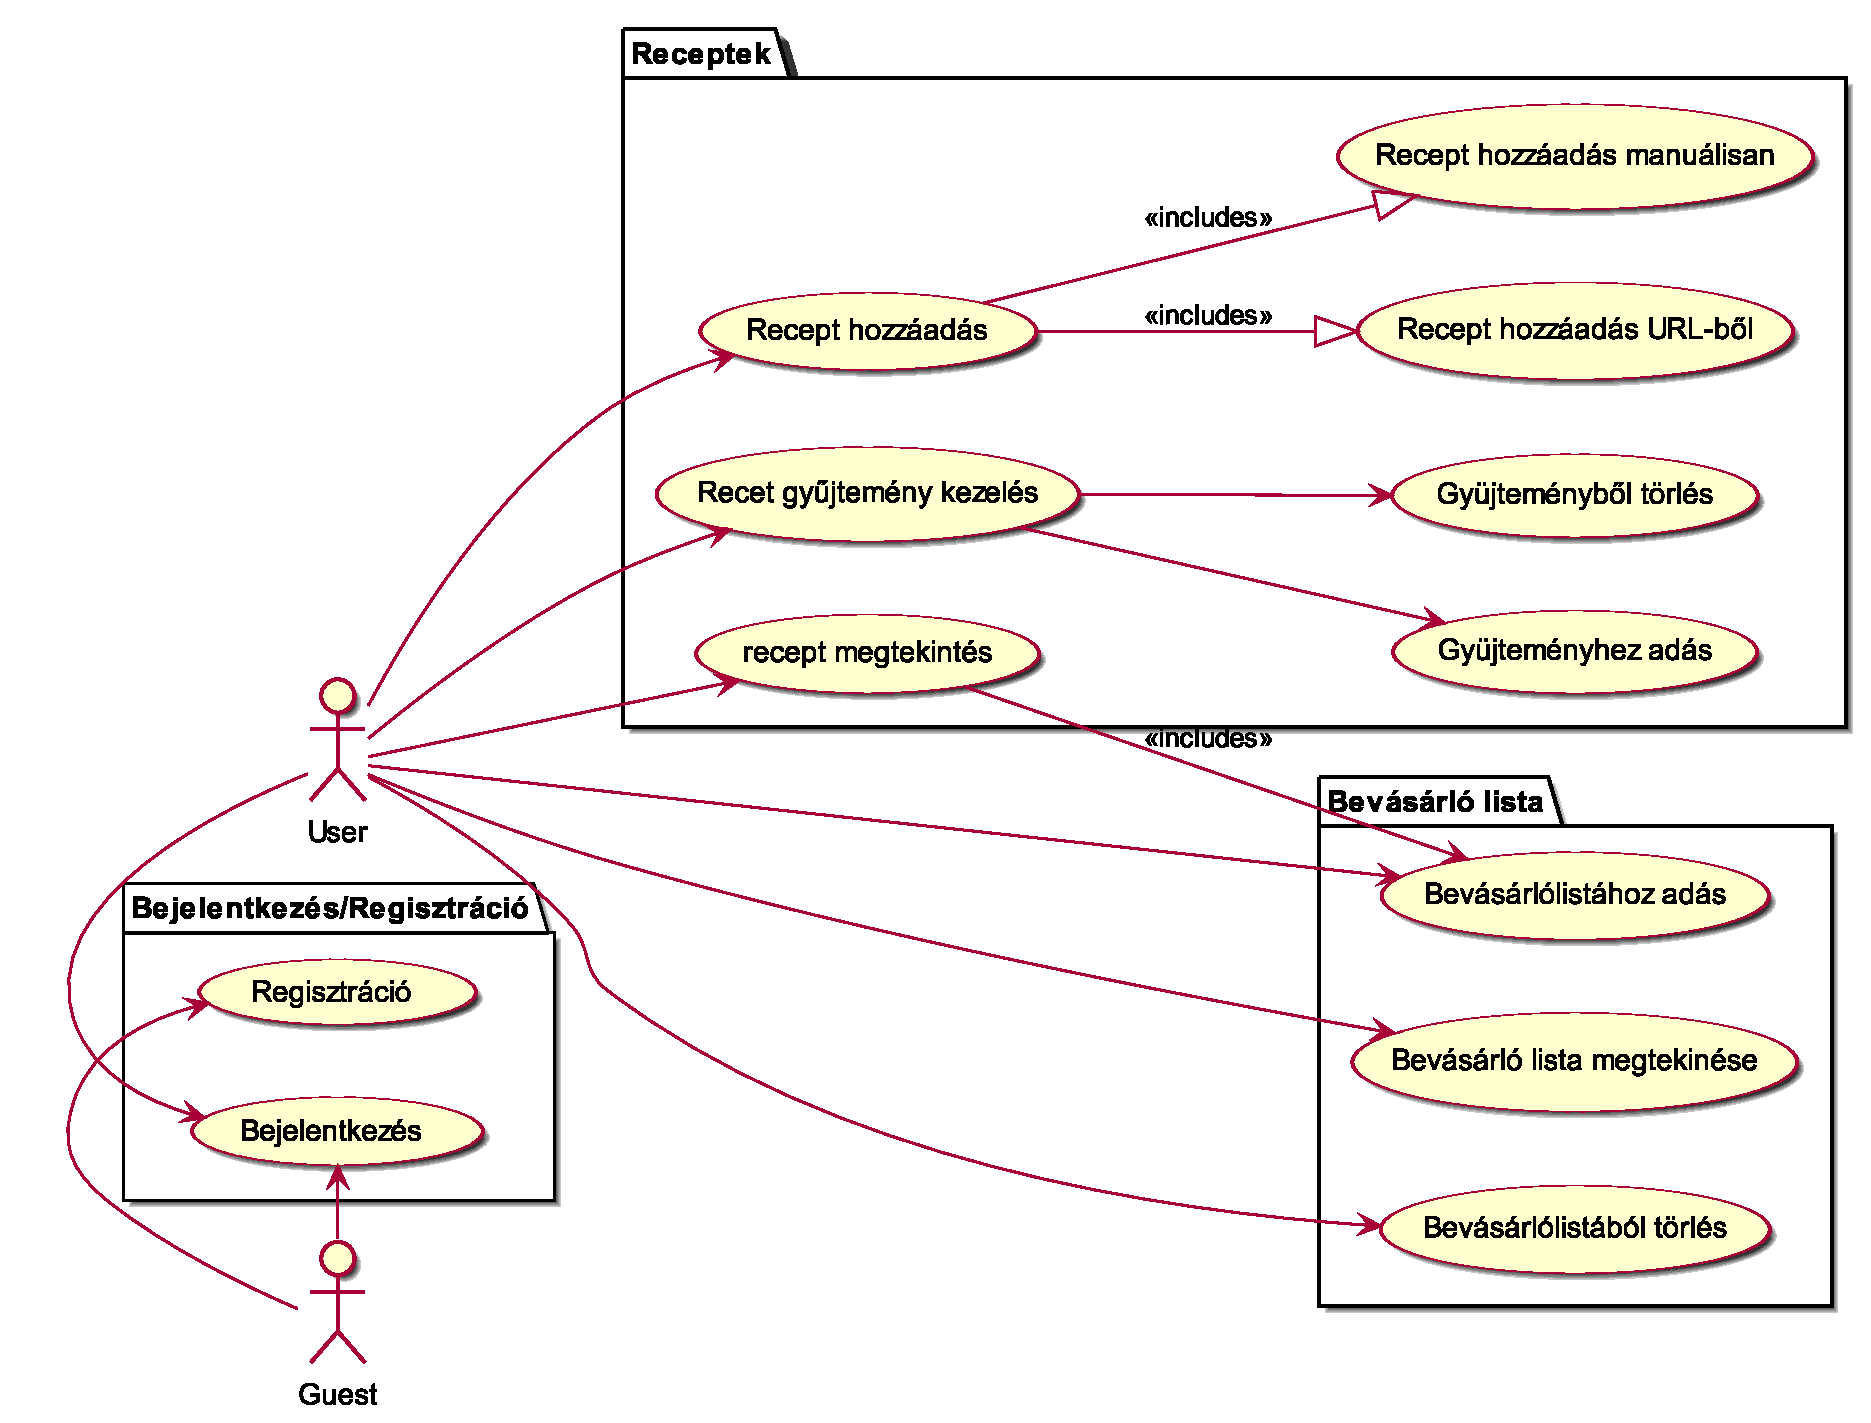
\includegraphics[scale=0.4]{out/diagrams/useCase/use-case.eps}
\begin{figure}[h]
	\centering
	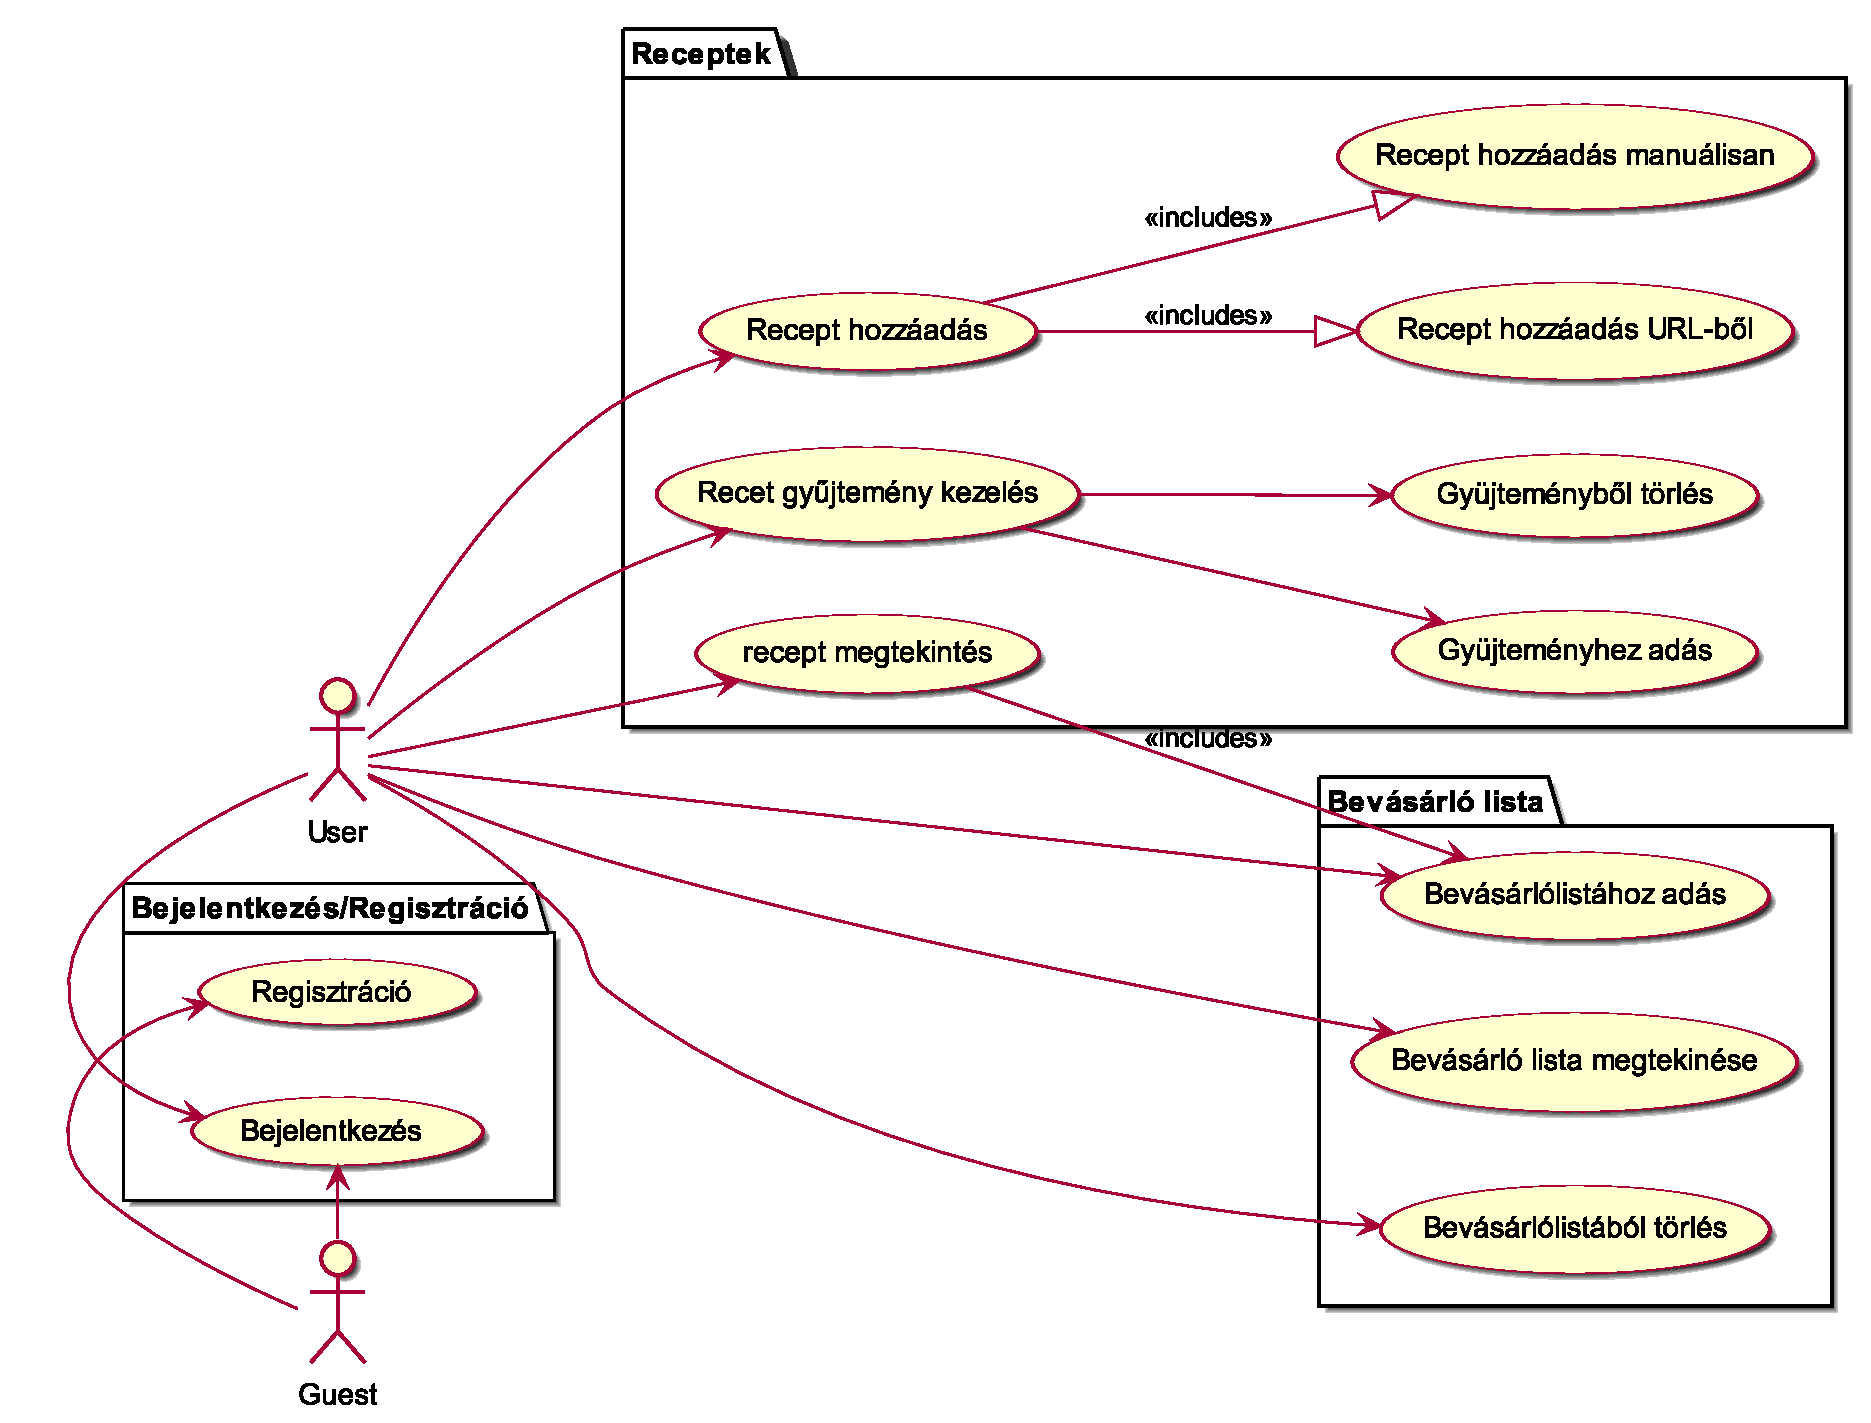
\includegraphics[width=\textwidth]{out/diagrams/useCase/use-case.eps}
	\caption{UseCase diagram}
    \label{fig:useCase}
\end{figure}


\section{Bejelentkezés/Regisztráció}
A weblap használatához be kell jelentkezni vagy regisztrálni kell. Ameddig ez nem történik meg, a felhasználó vendég státuszban van (lásd: \ref{fig:useCase}-es ábra “Vendég”). 

A regisztrációra két lehetőség van. Egyrész a regisztrációs oldalon a mezők (pl.: név, születési év, email, stb) kitöltésével tud manuálisan regisztrálni (lásd: \ref{fig:useCase}-es ábra “Regisztráció manuálisan”). Ekkor a rendszer az azonosításra a megadott email címet használja és ezt kell megadni a jelszavával együtt a belépéskor. Másrészt, ha a vendégnek van Google fiókja, akkor egyszerűen egy lépéssel azonnal regisztrálhat annak felhasználásával (lásd: \ref{fig:useCase}-es ábra “Regisztráció Google fiókkal”).

A bejelentkezésnél a regisztrációhoz hasonlóan két lehetőség áll rendelkezésre. Attól függően, hogy a felhasználó mely módszerrel regisztrált, az annak megfelelő módszerrel kell belépnie. Tehát, ha manuálisan regisztrált, akkor meg kell adni a regisztrációkor használt email címet és jelszót (lásd: \ref{fig:useCase}-es ábra “Bejelentkezés manuálisan”). Amennyiben Google fiókot használt a regisztrációhoz, akkor egyszerűen a “Sign In with Google” gombra kattintva tud belépni (lásd: \ref{fig:useCase}-es ábra “Bejelentkezés Google fiókkal”).


%\noindent
%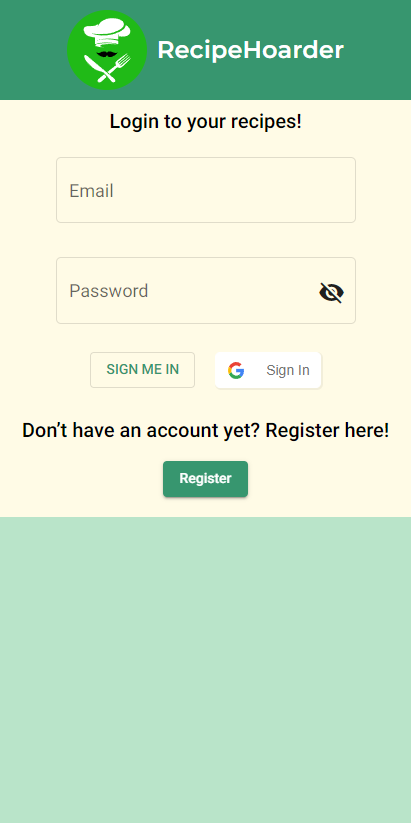
\includegraphics[scale=0.5]{pictures/mobil_login.png}
%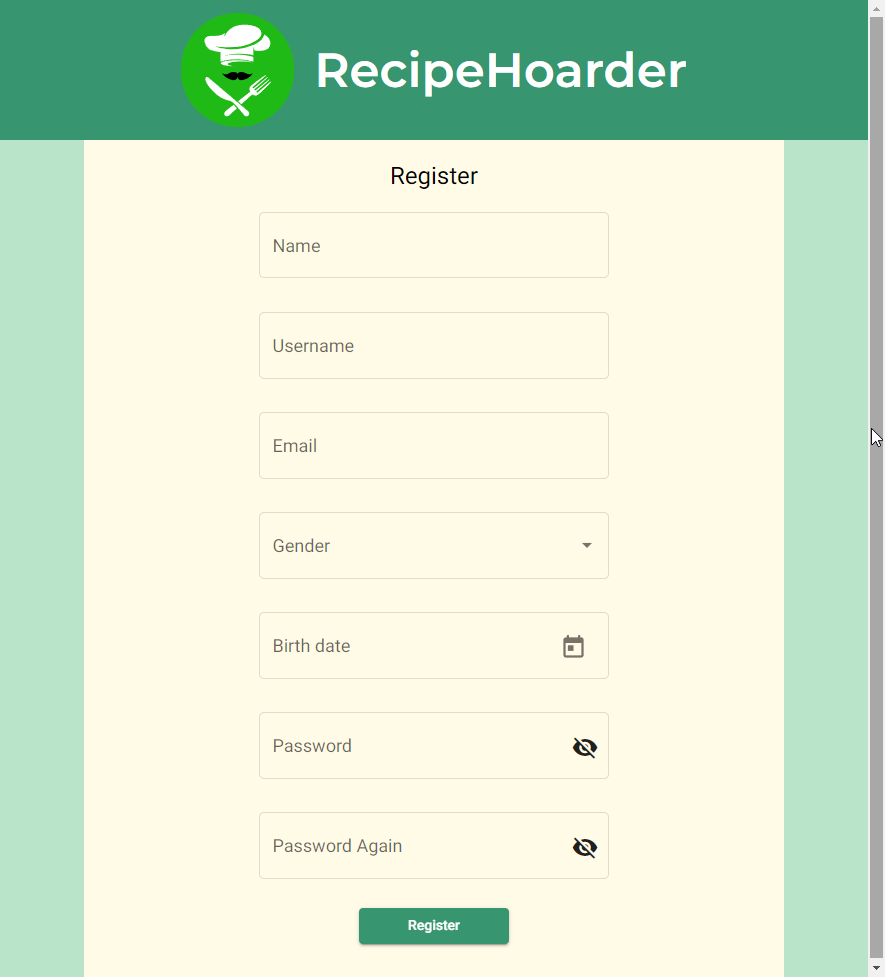
\includegraphics[scale=0.4]{pictures/web_register.png}

\section{Receptek}
A következőkben a receptekhez kapcsolódó főbb funkciókról lesz szó. Ez az ábrán a “Receptek” csoportban található felhasználási eseteket jelenti. Ezen funkcionalitások alkotják az alkalmazás legfontosabb képességeit. A piackutatásban megállapított fontos funkciókat tartalmazza, például a legfontosabbnak megállapított recept importálást.
%\noindent
%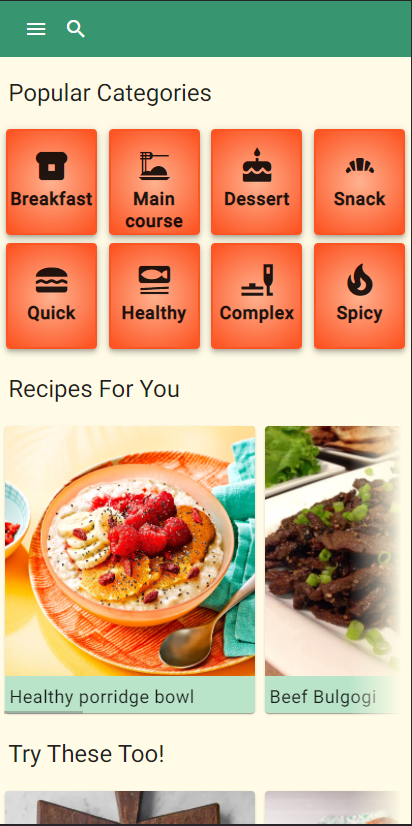
\includegraphics[scale=0.5]{pictures/mobil_home.png}


\subsection{Receptek hozzáadása} 
A weblap egyik jellegzetes alapfunkciója, hogy a közösség tölti fel az adatbázist receptekkel. Ez azért fontos, mert így nem az adminisztrátoroknak kell folyamatosan dolgozni, hogy minél több recept legyen elérhető a felhasználók számára. 

Egy recept feltöltésre két lehetőség is van. Az egyik az, hogy a felhasználó manuálisan tölti ki a recept paramétereit (lásd: \ref{fig:useCase}-es ábra “Recept hozzáadás manuálisan”). Ez azokban az esetekben fontos a felhasználó számára, amikor a recept nem az internetről származik, hanem például nyomtatott receptkönyvből vagy családi hagyományból. 

A másik opció az, hogy egy másik recepteket tartalmazó weboldal URL címét kimásolja a böngészőből és beilleszti a linket a RecipeHoarder importáló felületére (lásd: \ref{fig:useCase}-es ábra “Recept hozzáadás URL-ből”). Itt, amennyiben a forrás weblap támogatott, a program betölti a recept adatait. Ezután a felhasználónak lehetősége van módosítani a receptet, majd azt kinentve hozzá adni a globális recept lisához.

Mindkét opció során a felhasználónak meg kell adnia, hogy a recept mely előre meghatározott csoportba tartozik (Pl.: Reggeli, Csípős, stb.). Majd a kimentés után a rendszer mind a két módszernél megpróbál egy kalória mennyiséget számolni a recepthez.


\subsection{Receptgyűjtemény kezelés}
Ahhoz, hogy a weblap könnyen használható legyen, szükségünk van arra, hogy a felhasználó ki tudjon menteni recepteket egy saját gyűjteménybe. Ez nagyban megkönnyíti a recept későbbi megtalálását. Erre két különböző gyűjtemény áll a felhasználó rendelkezésére. Egyik a saját “receptkönyv”, amibe akárhány receptet kimethet, illetve a kedvencnek ítélt receptek gyűjteménye. A felhasználó bármely megtekintett vagy frissen beimportált receptet ki tud menteni a recept könyvébe (lásd: \ref{fig:useCase}-es ábra “Gyűjteményhez adás”), majd innen, amennyiben tetszett neki, hozzá tudja adni a kedvencekhez. Ez azt jelenti, hogy a kedvencekhez való hozzáadáshoz először ki kell menteni  a saját receptkönyvbe.

Természetesen a felhasználó bármikor meg tudja tekinteni az összes receptet, amit a saját receptkönyvbe vagy kedvencek közé mentett ki (lásd: \ref{fig:useCase}-es ábra “Gyűjtemény megtekintése”). Majd amennyiben egy receptet már nem szeretne az adott listában látni, akkor képes a receptet kivenni a kedvencek/saját receptkönyvből, de ezzel nem törlődik a globális receptlistából, így a többi felhasználó számára elérhető marad (lásd: \ref{fig:useCase}-es ábra “Gyűjteményből törlés”). 


\subsection{Recept megtekintés}
Mivel ez egy recept gyűjtő webes alkalmazás, ezért egyértelműen lehetőséget kell adni arra, hogy a receptek leírását meg lehessen tekinteni. Itt már megtalálható az összes eltárolt adat a receptről, mint például a elkészítési idő (ha van), kalória (ha van), hozzávalók vagy elkészítési lépések (lásd: \ref{fig:useCase}-es ábra “Recept megtekintés”).

\subsection{Receptre szűrés}
A weblapon van lehetőség keresni a receptek között, ezen belül is két mód van erre. Egy általános névre való keresés, valamint kategória szerint is lehet szűrni. Mivel egy recept létrehozásakor kötelező megadni legalább egy kategóriát, így egyszerűen kereshetők ez alapján.

Ez \az{\ref{fig:useCase}-es ábra} “Receptek” csoport alatt, a “Receptre szűrés”-nek felel meg a két lehetséges verziójával, “név szerinti” és “kategória szerinti” szűrés.


\subsection{Hibás recept jelentése}
Korábban volt szó arról hogy, az oldal adatbázisa a közösség által feltöltött receptek alapján nő. Ezért van arra lehetőség, hogy akár az importálás során különböző hibák keletkezzenek, amit a felhasználó nem vesz észre vagy nincs kedve kijavítani. Akár arra is van lehetőség, hogy támadás érje a weblapot, és keletkezzenek olyan receptek, amelyek hibásak. Ennek javítása érdekében minden recepthez tartozik egy hiba bejelentő rész, ahol előre megszabott lehetséges hibák listájából választva jelezhet a weblap karbantartóinak, hogy ha valami nem jó a recepten. Ezen lehetséges hibák közé tartozik például, ha hiányos az alapanyagok listája vagy trágár szavakat tartalmaz.

Ez \az{\ref{fig:useCase}-es ábra} “Receptek” rész alatt, a “Recept megtekintés”-hez tartozik “Hibás recept jelentés” néven.


\section{Bevásárló lista}
Minden felhasználónak van saját bevásárlólistája, amibe össze tudja gyűjteni a számára szükséges alapanayagokat. Ez a lista szintén személyre szabott és csak a felhasználó látja, vagy módosíthatja.

\subsection{Bevásárló listához adás}
A listához adásra két lehetőség van. A szokásos bevásárlólista módszert követve manuálisan is ki lehet tölteni az adatokat, majd a listához adni. A másik módszer a recepteken belül, a felsorolt alapanyagokat is egyesével hozzá lehet adni illetve a recepteknél lehetőség vagy az összes alapanyagot azonnal hozzáadni a listához.

Ezen a diagramon a “Bevásárlólista” rész alatt, a “Bevásárló listához adás” résznek felel meg.


\subsection{Bevásárló lista megtekintés}
A bevásárlólista megjelenítésénél a korábban hozzáadott alapanyagok vannak felsorolva. A bevásárlólista az alapanyagokat a hozzáadásuk dátuma szerint jeleníti meg. Igy könnyen követhető mikor egy új tétel lett a listához adva.  Amennyiben az alapanyagnak nincs mértékegysége vagy mennyisége, akkor azok az adatok nem lesznek megjelenítve, hogy elkerüljük, hogy például “0 pasta“ legyen megjelenítve.

Ezen az ábrán a “Bevásárlólista” rész alatt lévő “Bevásárló lista megtekintése” résznek felel meg.


\subsection{Bevásárló listából törlés}
Ha a felhasználónak már nem kell egy adott alapanyag a listából, legyen ez azért, mert már megvette vagy csak nem aktuális már, akkor könnyen egy kattintással el lehet tüntetni a listából. Másik verzió a lista ürítésére a lista alatt lévő gomb megnyomásával az egész lista törlése. Így gyorsan és egyszerűen lehet újrakezdeni a lista használatát anélkül, hogy az összes elemet egyesével kellett volna törölni.

Ezen az ábrán a “Bevásárlólista” rész alatt lévő “Bevásárló listából törlés” résznek felel meg.

%\noindent
%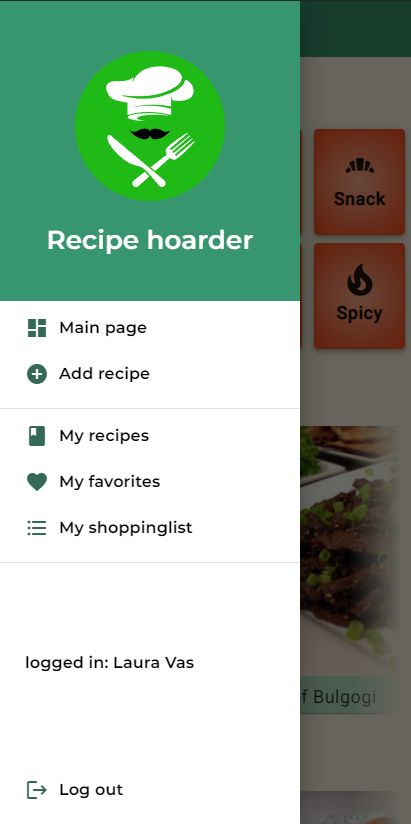
\includegraphics[scale=0.5]{pictures/mobil_menu.png}
%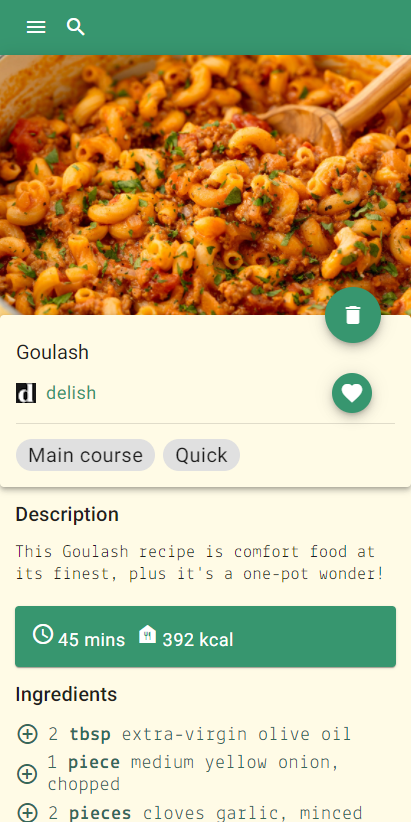
\includegraphics[scale=0.5]{pictures/mobil_recipe-top.png} \\
%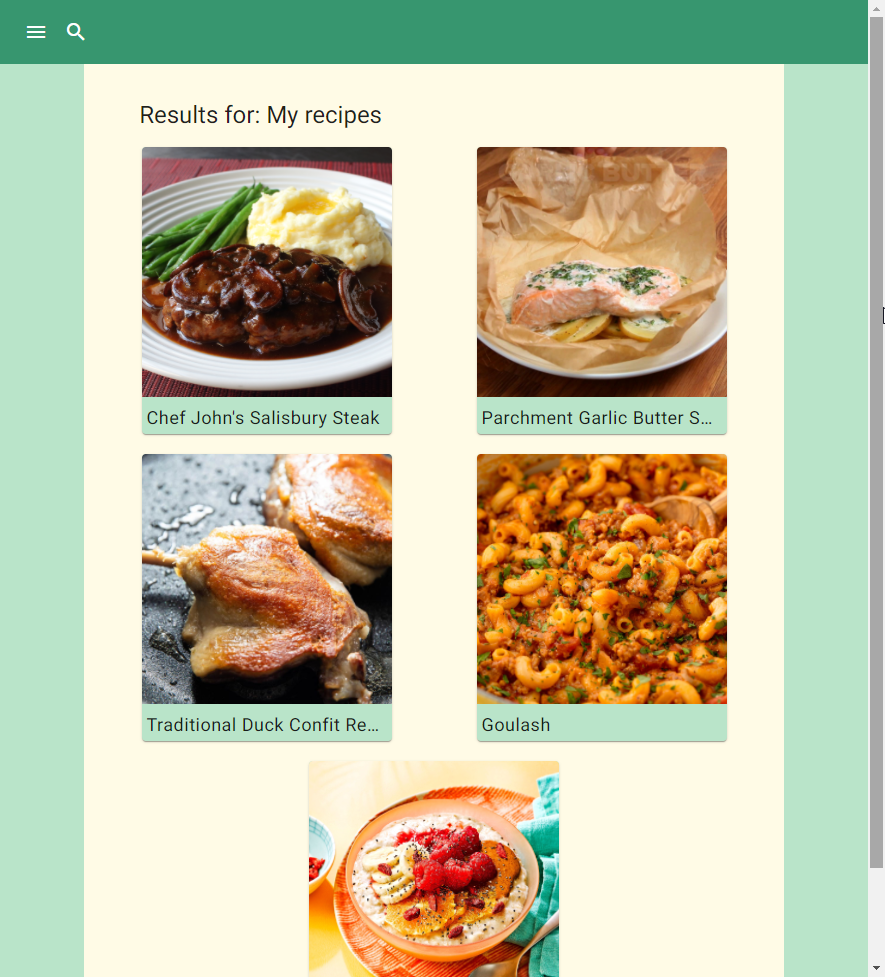
\includegraphics[scale=0.4]{pictures/web_recipeCollection.png}

%\noindent
%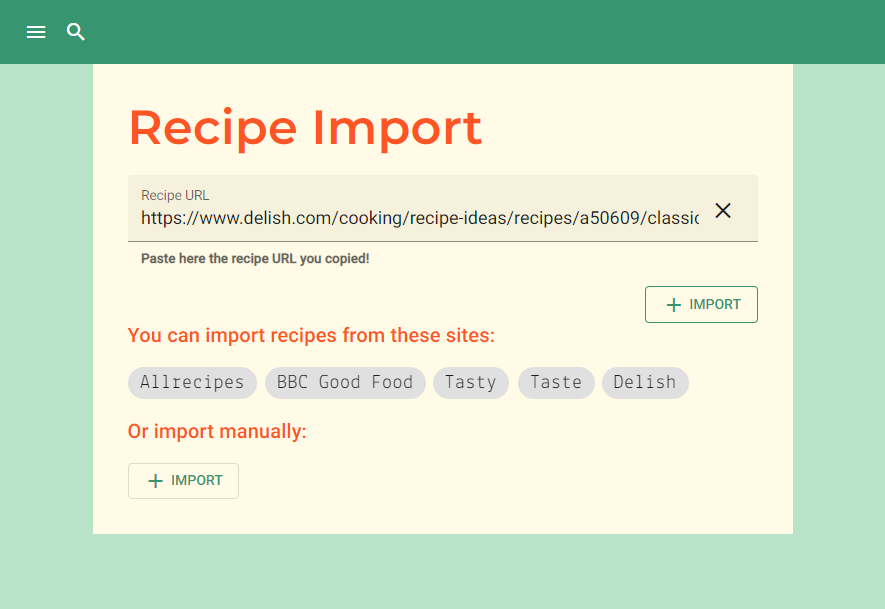
\includegraphics[scale=0.4]{pictures/web_import.png}
%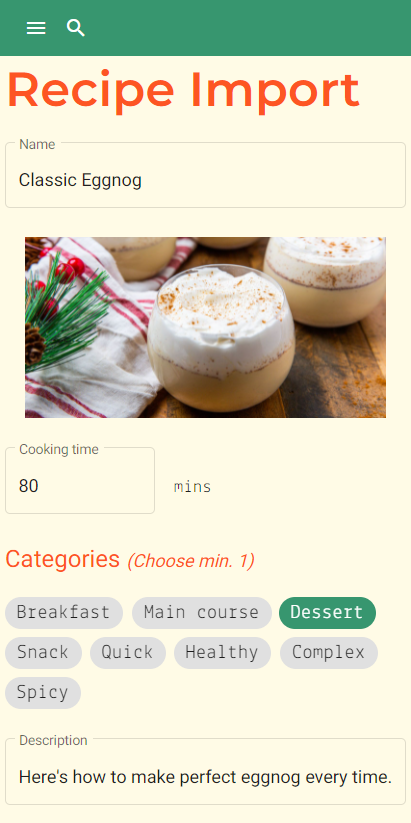
\includegraphics[scale=0.5]{pictures/mobile_importDataCheck.png}

%\noindent
%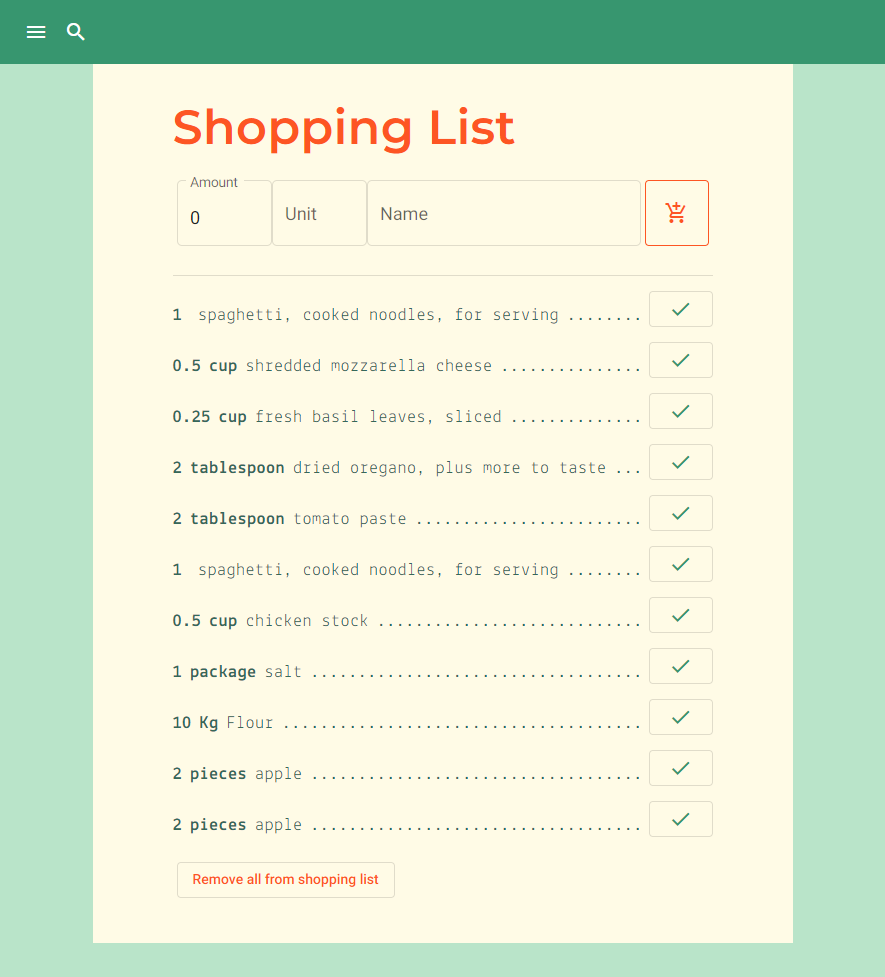
\includegraphics[scale=0.4]{pictures/web_shoppinglist.png}

%\noindent
%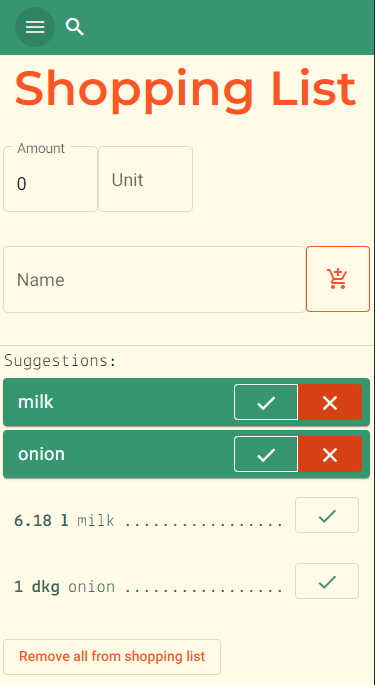
\includegraphics[scale=0.5]{pictures/mobile_suggestion.png}

\chapter{Felhasznált technológiák}
Itt fogom részletezni a kiemeltebb felhasznált technológiákról alapvető információkat, valamint szerepüket ebben a projektben.

\section{Angular}
Egy TypeScript alapú Framework, amit  eredetileg a Google fejlesztett ki, de most már nyílt forráskódú. Az Angular egy teljes újraírása a régi AngularJS-nek. Egyik legnagyobb előnye, hogy komponens alapú keretrendszer, ami segítségével újra felhasználható kódot lehet írni. Támogatja a Single Page alkalmazás készítését. Ezeken a weblapokon a weblap újratöltése nélkül tud a felhasználó navigálni, ezzel is gyorsabbá téve azt.

A felhasználói felület tervezése során is igyekeztem komponenseket kialakítani mind telefonos mind desktopos kinézetben. A komponensekkel való munka megkönnyíti egy projekt fejlesztését, mivel akár saját fejlesztésből, akár külső könyvtárból szerzett elemeketből lehet egyszerűen felépíteni a weblapokat. Ezeknek az elemeknek másik nagy előnye, hogy elég csak az eredetit módosítani ahhoz, hogy mindenhol megváltozzon, ezzel is egységesítve az oldal szerkezetét, valamint segítve a fejlesztők dolgát.


\section{Angular Material}
Az Angular Material egy a Google által fejlesztett komponens csomag. Ez segít a fejlesztőknek már kész és modern dizájnos komponenseket egyszerűen felhasználni a projektekben. Ez elsősorban egy UI komponens dizájn könyvtár, ami importálás után egyszerűen használható. A weboldalán pedig példákkal és részletes dokumentációval fel vannak sorolva a létező komponensek és ezek különböző változatai.

Az én projektem is nagy részben ennek a könyvtárnak a komponenseit használja fel. Csak pár helyen kellett kiegészíteni a már létező verziót, hogy illeszkedjenek az eredeti tervekhez. Ezen felül a projekt témája is az Angular Material alapján lett felépítve, hogy a komponenseknek könnyen meglehessen adni az alap színeket és tipográfia szabályokat


\section{FireBase}
Eredetileg független cég által fejlesztett de most már a Google által fejlesztett webes és mobilos alkalmazások készítéséhez létrehozott platform. Manapság nagyon népszerű az egyszerűsített adatbázis felépítése valamint a könnyű és könnyen értelmezhető kezelő felülete miatt. Arról nem is beszélve, hogy rengeteg dokumentáció létezik a fejlesztők számára.

Ebben a projektben elég sok helyen használom a Firebase funkcióit. Az egész weblap a Firebase Hosting felületéről működik, ami egy statikus weblap hosztolási felület. Ez a GitHub-bal össze van kötve, ha a Main Branch-re feltöltés történik, akkor a Firebase-re automatikusan feltöltődik az új production verzió.

A FireStore Database-t használom a weblap adatainak tárolásához. Itt vannak eltárolva  receptek, felhasználók, felhasználókhoz különböző kollekciók és bevásárló listájuk és meta adatok. A Cloud FireStore-on belül lehet beállítani az adatbázis Rule-okat. Ezt azt jelenti, hogy be lehet állítani, hogy különböző kollekciókat kik érhetnek el, milyen tevékenységek vannak engedélyezve nekik, valamit, hogy milyen jogokkal milyen adatbázis műveleteket lehet csinálni. 

A FireBase Storage-ban tárolódnak a receptekből kimentett képek, amik az importálás során kerülnek az adatbázisba.

A legnagyobb biztonság érdekében a Firebase Auth-ot használom a weblap bejelentkezés és regisztrációs műveleteihez. Így lehetséges email és jelszó párossal regisztrálni majd bejelentkezni, viszont, akinek van Gmail fiókja annak lehetősége van egy lépésben azonnal regisztrálni és belépni annak segítségével.

A recept importálás és a bevásárlólista egy része a Firebase Cloud Function keresztül szerver oldalon fut. Ez nem csak olcsóbb, mivel szerver oldali adatbázis lekérdezések ingyenesek a kliens oldalival szemben, hanem az importálás során felmerült problémát is megoldotta. Ez a  probléma az, hogy egy honlap nem kérdezhet le adatot egy másikról kliens oldalon keresztül, mivel a cél weblapok CORS beállítása ezt nem engedi. Azon kívül, mikor a bevásárló listába új alapanyag kerülnek, akkor egy trigger leful a szerver oldalon, ami segítségével állítjuk elő az ajánlóhoz a metaadatokat.


\section{PWA}
PWA azaz Progressive Web Application egy koncepció, amit követve lehetséges megbízható, stabil és telepíthető webes applikációkat fejleszteni. Az alap szabályait követve a weblap akár platformspecifikus alkalmazássá is alakítható. A PWA lehetővé teszi az alkalmazások használatát bárhol, bármikor, bármilyen eszközön. 

A projekt esetében az Angular-t kell kiegészíteni JavaScript kóddal, hogy ha az eszköznek nincs internet elérése, akkor a script segítségével a localstorage-ba elmentett változatát használja a weblapnak. Ezzel elérhető, hogy valamilyen szinten használható legyen a weblap offline környezetben is. Szerencsére mind az Angular, mind an Firebase úgy lett kifejlesztve, hogy csak egy-egy helyen kell megadni neki, hogy az Angular Service Worker-t használja, ezért nekem nem kellett saját kódot írni ahhoz, hogy internet nélkül is használható legyen a weblap. Ez persze limitált arra, ami cachelve lett, például a keresés csak a már egyszer letöltött receptekre fog működni, de a bevásárló listához adás során, mikor az eszközön újra lesz internet, az egész szinkronizálódik, hogy ne legyen adatvesztés.

\section{Schema.org}
A shema.org egy weblap, ami azért készűlt, hogy a közösség a központosított sémákat használja különböző weblapokon, e-mailekben, modellekben, adatbázisok tervezésében vagy sok más helyen. Sok különböző kódolással használható, de a legnépszerűbbek a JSON-LD, Microdata valamint a RDFa. Ezek a szótárak olyan entitásokat és kapcsolatokat írnak le, amik segítik a fejlesztők számára a megfelelő sémát kiválasztani. Tehát összességében, ez egy tervgyűjtemény.

A projektben fontos szerepet játszott a shema.org által biztosított “Recipe” séma feldolgozása és megértése, mivel a recept importálás más weblapokról ezen alapul. A jól felépített weblapok manapság tartalmaznak egy vagy több JSON-LD meta információt, amiben a weblapon jelenleg megjelenő adatok vannak eltárólva JSON formátumban a Shema.org szerinti felépítés alapján.

\section{Figma}
Egy  vektorgrafikus szerkesztő, ahol felhasználói felület prototípusokat lehet tervezni. A program legfőképp webalapú, de letölthető desktopos verziója is. A program képes a tervezett lapok élő tükrözésére akár saját telefonon az applikáción keresztül, vagy csak az emuláló felületen keresztül. A figma egy modern dizájn tervező app, amiben egyszerűen fel lehet használni a material design stílust és alap komponenseket, ezzel is segítve az Angular-ban is használt komponens alapú gondolkodást. Másik nagy előnye, hogy interaktívvá lehet tenni a tervezés során a gombokat, komponenseket, így akár a teljes felhasználói élmény kipróbálható. Valamint a kész dizájnoknak meglehet nézni a pontos CSS stílus kódját is, ezzel is segítve a konkrét kódolás folyamatát.

Ez a program sokat segített a tervezésben, mivel a kész material design komponenseket tudtam próbálgatni anélkül, hogy először mélyebben tanulmányoznám az Angular felépítését. Az egységes dijájn és téma tervezésében pedig segített konzisztensnek maradnom. Ez igaz mint a színekre, mind a tipográfiára.




\chapter{A rendszer magas szintű áttekintése}
Mint minden más webes alkalmazás, ez a projekt is egyértelműen felbontható két fő egységre a szerver és a kliens oldal mentén. A kliens oldal azt a kódot és egyéb fájlokat jeleni, amiket az interneten keresztűl a felhasználó böngészője tölt le és futtat. Míg a szerver oldali kód az egy központi helyen fut és a hosszabb időt igénybe vevő számításokat, illetve az adatbázis elérését végzi.

\noindent
\begin{figure}[H]
	\centering
	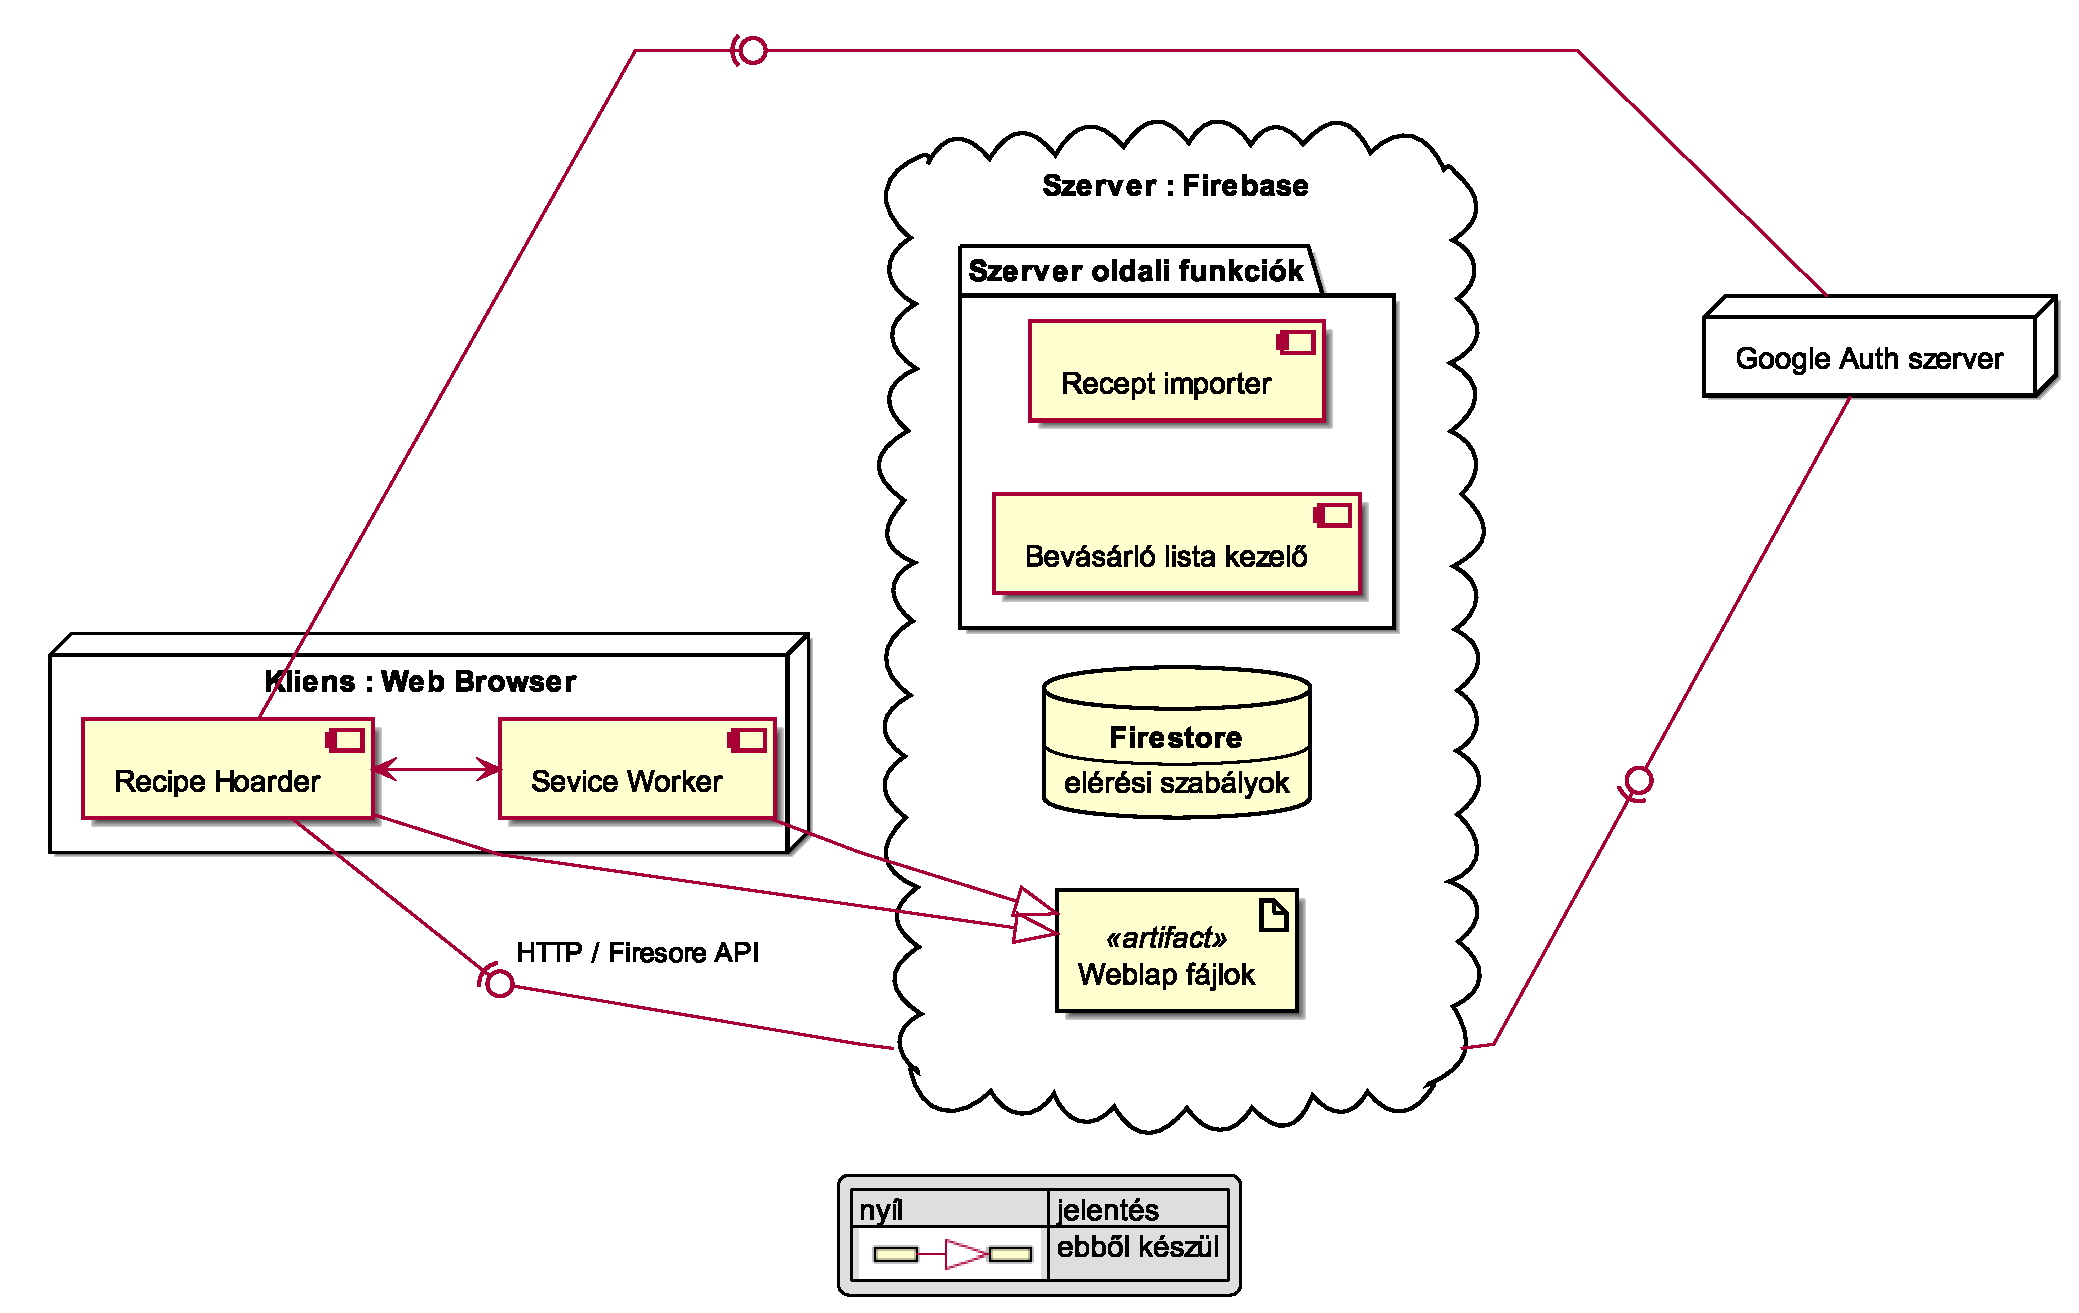
\includegraphics[width=\textwidth]{out/diagrams/deployment/deployment.eps}
	\caption{Diagram a kilens és szerver oldali összeköttetésről}
    \label{fig:deployment}
\end{figure}

\section{Szerver oldal}
A projekt esetében a szerveroldali ufnkcinalitásokat a FireBase segítségével lett megvalósítva. Ez nagyban megkönnyítette a munkát, mivel a szerver tényleges működtetését a FireBase végzi. Az adatbázis szerepét a FireBase FireStore tölti be, ami egy NoSQL alapú adatbázis (lásd: \ref{dataSchemes}. fejezetben részletesebben).  Ez egy biztonságos kliens oldalról is használható API-val rendelkezik, aminek segítségével az adatbázis műveletek elvégzéséhez nincs szükség saját szerver oldali kód írására. A weblap statikus fájljainak kiszolgálására a FireBase Hosting van használva Aminek segítségével nincs szükség saját Apache vagy NGINX szerver üzemeltetésére. Ahol szükséges volt szerver oldalon saját kódot futtatni, ott a FireStore által nyújtott Cloud Functions megoldást használtam.

\subsection{Firebase functions}
A Firebase functions egy olyan felhő alapú megoldás, ahol a fejlesztőnek csak a ténylegesen futtatni kívánt kódot kell megadnia a virtuális gép, az azon futó operációs rendszer és a program elindítása mind a platform által van kezelve. Ez nagyban megkönnyíti a fejlesztést, mivel nem kell plusz időt fordítani a szerver karbantartására. A Firebase csak JavaScript/TypeScript -ben írt kódot tud futtatni. Mivel a kliens oldal is TypeScript-ben készűlt, ezért bizonyos funkciókat, illetve adatstruktúrákat a két komponens között meglehet osztani. 

Az általunk megírt programokat többféle események is elindíthatják. Leggyakoribb példák erre a bejövő HTTP kérések vagy az adatbázisban történt változások. Ezek közül a projekt mind a kettőt használja.

\subsection{Főbb funkciói és célja}
A szerver oldalon két fő funkcionalitást kellett megvalósítani. Első és legfontosabb a receptek importálásáért felelős Cloud Function. Ez a kliens által küldött speciális HTTP üzenetre indul el és végzi el a receptek letöltését és értelmezését. A második funkcionalitás a bevásárló lista ajánlóhoz metaadatok előállítását végzi, amit minden bevásárlólistához adáskor elvégez.

\section{Kliens oldali adatbázis műveletek}
Services...

\section{Bevásárlólista ajánló}
trigger és működés

%TODO: more?

\chapter{Architektúra}
\section{Bevásárló lista}
\begin{figure}%
    \centering
    \subfloat[\centering label 1]{{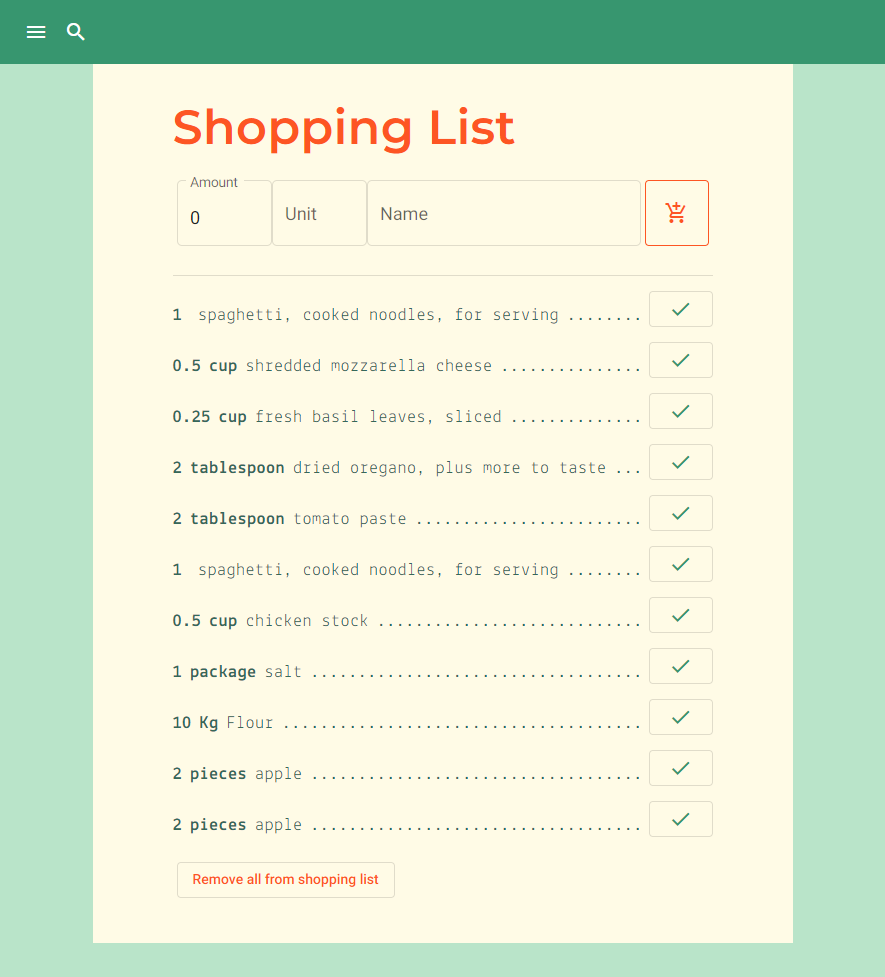
\includegraphics[width=5cm]{pictures/web_shoppinglist.png} }}%
    \qquad
    \subfloat[\centering label 2]{{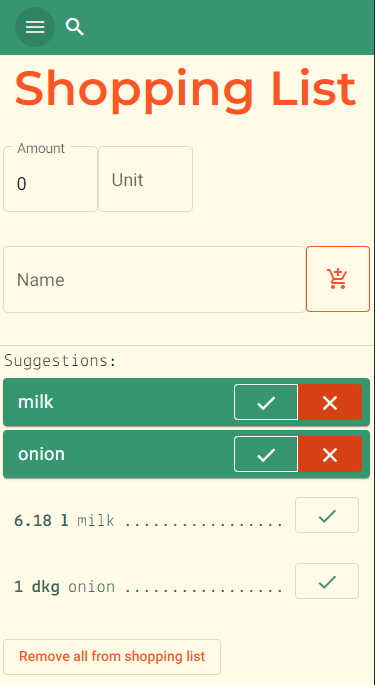
\includegraphics[width=5cm]{pictures/mobile_suggestion.png} }}%
    \caption{2 Figures side by side}%
    \label{fig:example}%
\end{figure}


\chapter{Adatmodellek}
\label{dataSchemes}
Az adatbázis felépítése különbözik a megszokott táblás módszertől, mivel a Firebase a NoSQL módszerrel tárolja az adatokat, amivel gyorsabb a keresés az adatok között. A szerkezete nagyon egyszerű, mivel csak egyszerű kollekciónkból és dokumentumokból áll, felépítése hasonlít a JSON fájltípusokra. Minden adat egy-egy dokumentumban tárolódik és ezek a dokumentumok vannak elrendezve kollekcióban. A szokványos SQL adatbázisoktól eltérően a FireStore-nak nincs fix sémája. Ez azt jelenti, hogy egy kollekción belül a dokumentumoknak felépítése nem rögzített. Így előfordulhat az, hogy egy dokumentumnak a többihez képes több vagy kevesebb adatja van. Emiatt a dokumentumok frissítésére külön energiát és figyelmet kell fordítani. Ezt a legtöbb esetben Cloud Functions futtatásával szokás megoldani.

A FireStore-ban a dokumentumok olyan felépítésű adattárolók, amelyekben egy tetszőleges szöveges kulcshoz tudunk valamilyen típusú adatot rendelni. Ezek az adatok lehetnek:
\begin{itemize}
	\item \textbf{Szöveg} (string), ami UTF-8 kódolású és maximum 1MiB méretű lehet
	\item \textbf{Szám} (number),  tetszőleges pontosságú számérték
	\item \textbf{Igaz/Hamis} (boolean), igaz vagy hamis
	\item \textbf{Tetszőleges adatstruktúra} (map), ez egy a JSON formátumhoz nagyban hasonlító kötetlen adatmező
	\item \textbf{Üres} (null)
	\item \textbf{Időpont} (timestamp), ez egy dátumot és másodpercre pontos időpontot jelez

	\item \textbf{Földrajzi koordináta} (geopoint), hosszúsági és szélességi fokot egy mezőben tároló típus

	\item \textbf{Referencia} (reference), másik dokumentumra mutató elérési út
	\item \textbf{Tömb} (array), egy különleges tároló, ami az eddig felsorolt összes típusból képes sokat eltárolni

\end{itemize}
 

\section{Recipes}
Az adatbázisban az egyik legfontosabb adatok a receptek, mivel ezekre épül az egész weblap témája. A receptek a feltöltés során automatikus azonosító ID értéket kapnak, ami a weblapon az URL címben az azonosításért is is felelős. A recepteket egy kollekcióban tároljuk és ezen belül a dokumentumok az adott recept adatait tartalmazzák, ezek közé tartozik például: kalória, teljes főzési idő (percben mérve), recept neve, eredeti URL, stb. Ezek az alap adatok, csak simán kulcs érték párok.

Alapanyagokon belül eltároljuk a mennyiséget, mértékegységet és az alapanyag nevét. Valamint a recept elkészítésének lépéseihez el tároljuk a sorrendbeli számát és a lépés leírását. Jelenleg még kulcs-tömb értékben vannak tárolva az alapanyagok és lépések, viszont a jövőben ez lehet megváltozik alkollekcióvá a gyorsabb betöltés idő eléréséért.


\noindent
\begin{figure}[H]
	\centering
	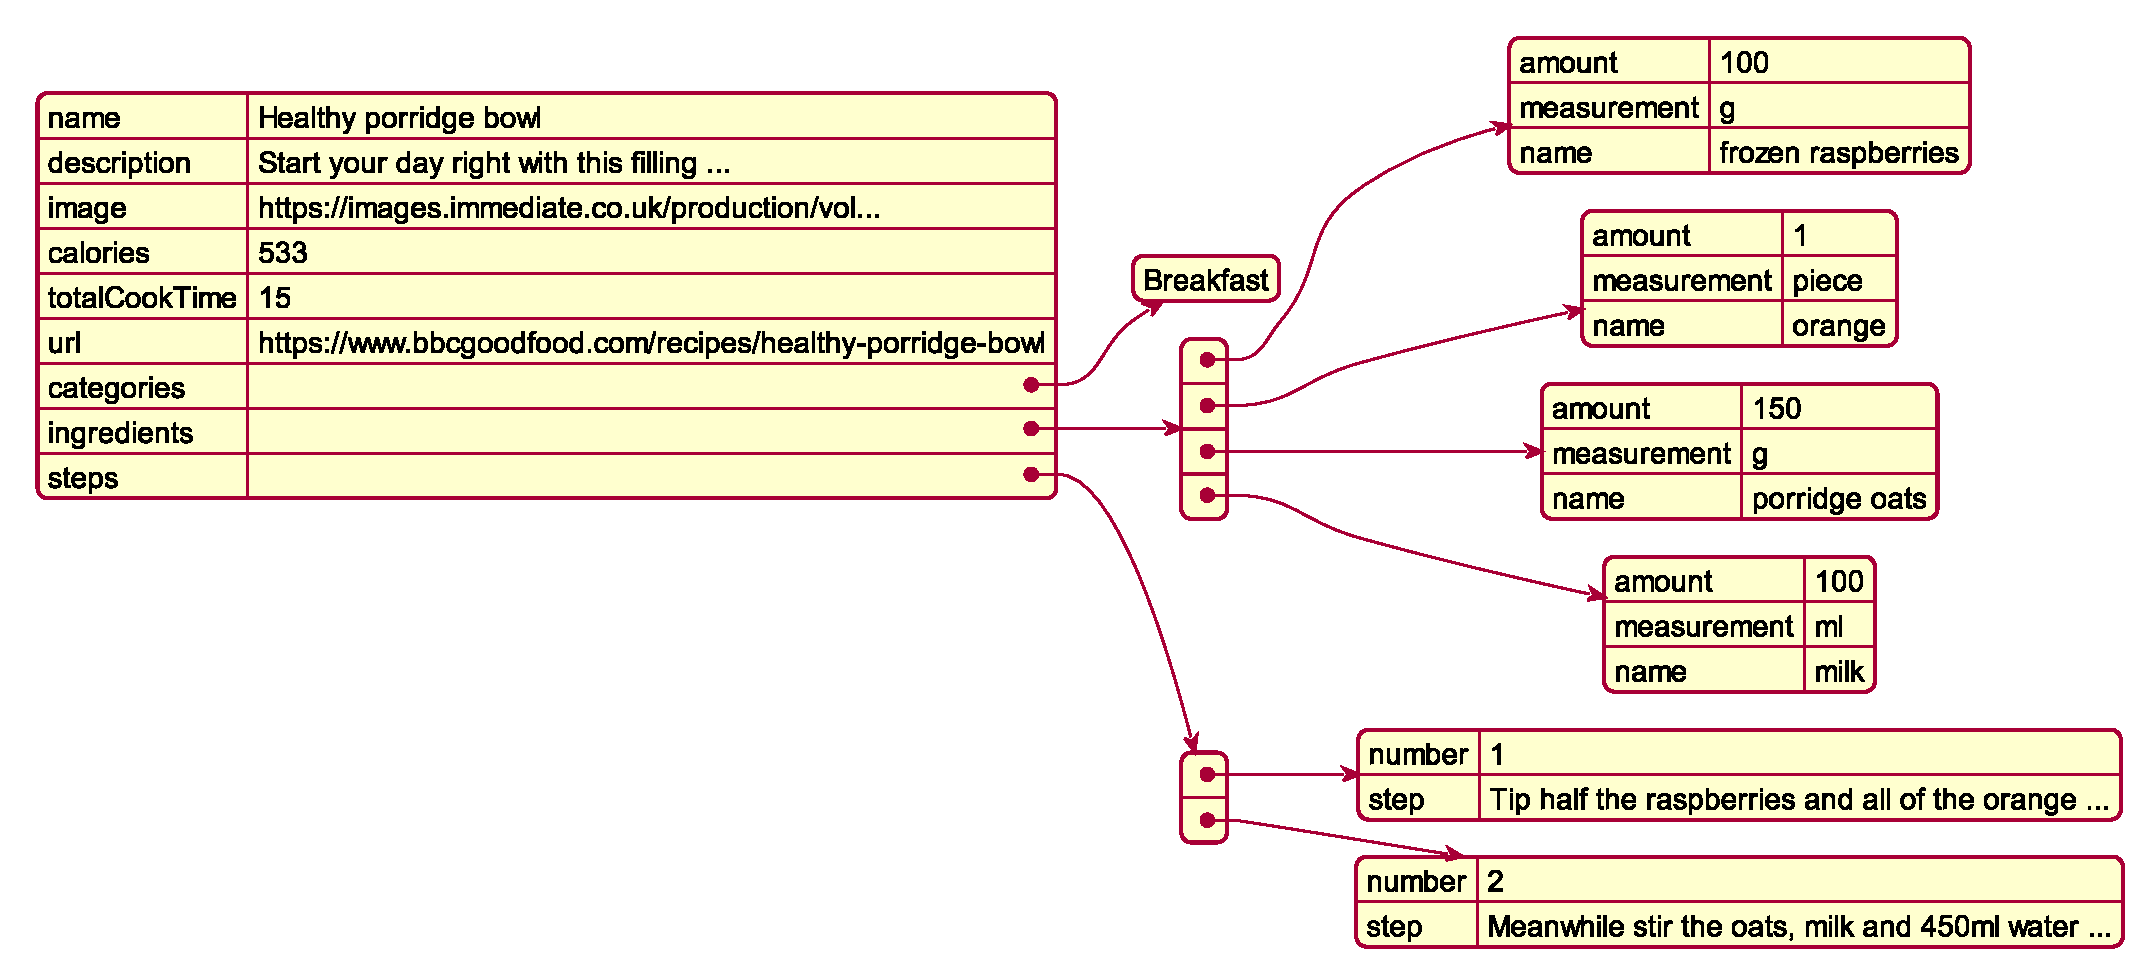
\includegraphics[width=\textwidth]{out/diagrams/jsonRecipes/jsonRecipes.eps}
	\caption{Minta a receptek adatbázis felépítéséről}
    \label{fig:jsonRecipes}
\end{figure}

\section{Users}
Az adatbázisban a felhasználókat egy kollekcióban tároljuk. A regisztráció során létrejön egy új dokumentum az adatbázisban. Itt tároljuk el az egyéb adatokat, amit a felhasználó az alap e-mail és jelszón kívül megad. Az egyéb adatok segíthetnek a jövőben személyre szabott recept ajánlót készíteni. 

Minden felhasználóhoz továbbá eltároljuk a Firebase Auth által adott “UID” azonosítót ami garantáltan egyedi.Itt a korábban említett kulcs-tömb típushoz képest már alkollekciók lettek bevezetve. Ezekbe az alkollekciókan tároljuk el a felhasználó által elmentett recepteket. Illetve hasonló módon tároljuk el a bevásárló lista adatait is.

Az alkollekció azért fontos ebben az esetben, mert amikor például le akarjuk kérdezni a felhasználó kedvenc receptjeit, akkor nem kell mindig az egész felhasználói adatot lekérdezni. Hanem lekérdezhető ugyanúgy, mint egy egyedülálló kollekció. Ezzel gyorsabb lesz a weblap, valamint spórolunk a fölösleges adatok kezelésével is. A felhasználó által a könyvtárába elmentett receptek, a felhasználó dokumentuma alatt lévő “base” al kollekcióban kerülnek el tárolásra. Ezek a recept ID-jét és a kimentési időpontot tartalmazó dokumentumokkal vannak eltárolva. Ugyanez igaz a kedvencek listára, ami a  “favourites” al kollekcióban van tárolva. Amint a felhasználó kimentett egy receptet a saját listájába, akkor van lehetősége ezt tovább elmenteni a kedvencek közé. Ez ugyanúgy működik mint a sima listába mentés. Amennyiben viszont a saját listájából törli a receptet, akkor a kedvencek közül is eltűnik. 

A bevásárló listába a mentés dátumát és a pontos adatokat is elmentjük az alapanyagról. A létrehozás dátuma a sorrendbe rendezés és a metaadat számítás miatt fontos. Ha a felhasználó úgy dönt, hogy az lista elem már nem aktuális, akkor az törölhető a listából. Illetve a bevásárló listáról el vannak tárolva meta adatok, amiket egy-egy termék kettő listához adása között eltelt időből számolunk ki. Az ajánló jelenleg csak az alapanyag nevét ajánlja fel, viszont a mértékegység és mennyiség is el van tárolva, ezt a jövőben pontosabb számításokra lehet felhasználni. Ezen kívül, mikor az adat létrejön, a “score” értéke 2. Ez egy érték, ami segít az ajánlás sikerességét követni, max értéke 5, minimum értéke 0. Végül a “nextDate” egy számolt TimeStamp érték, ami a eredeti hozzáadás dátumából és az újonnan hozzáadott alapanyag dátumából számolunk ki.


\noindent
%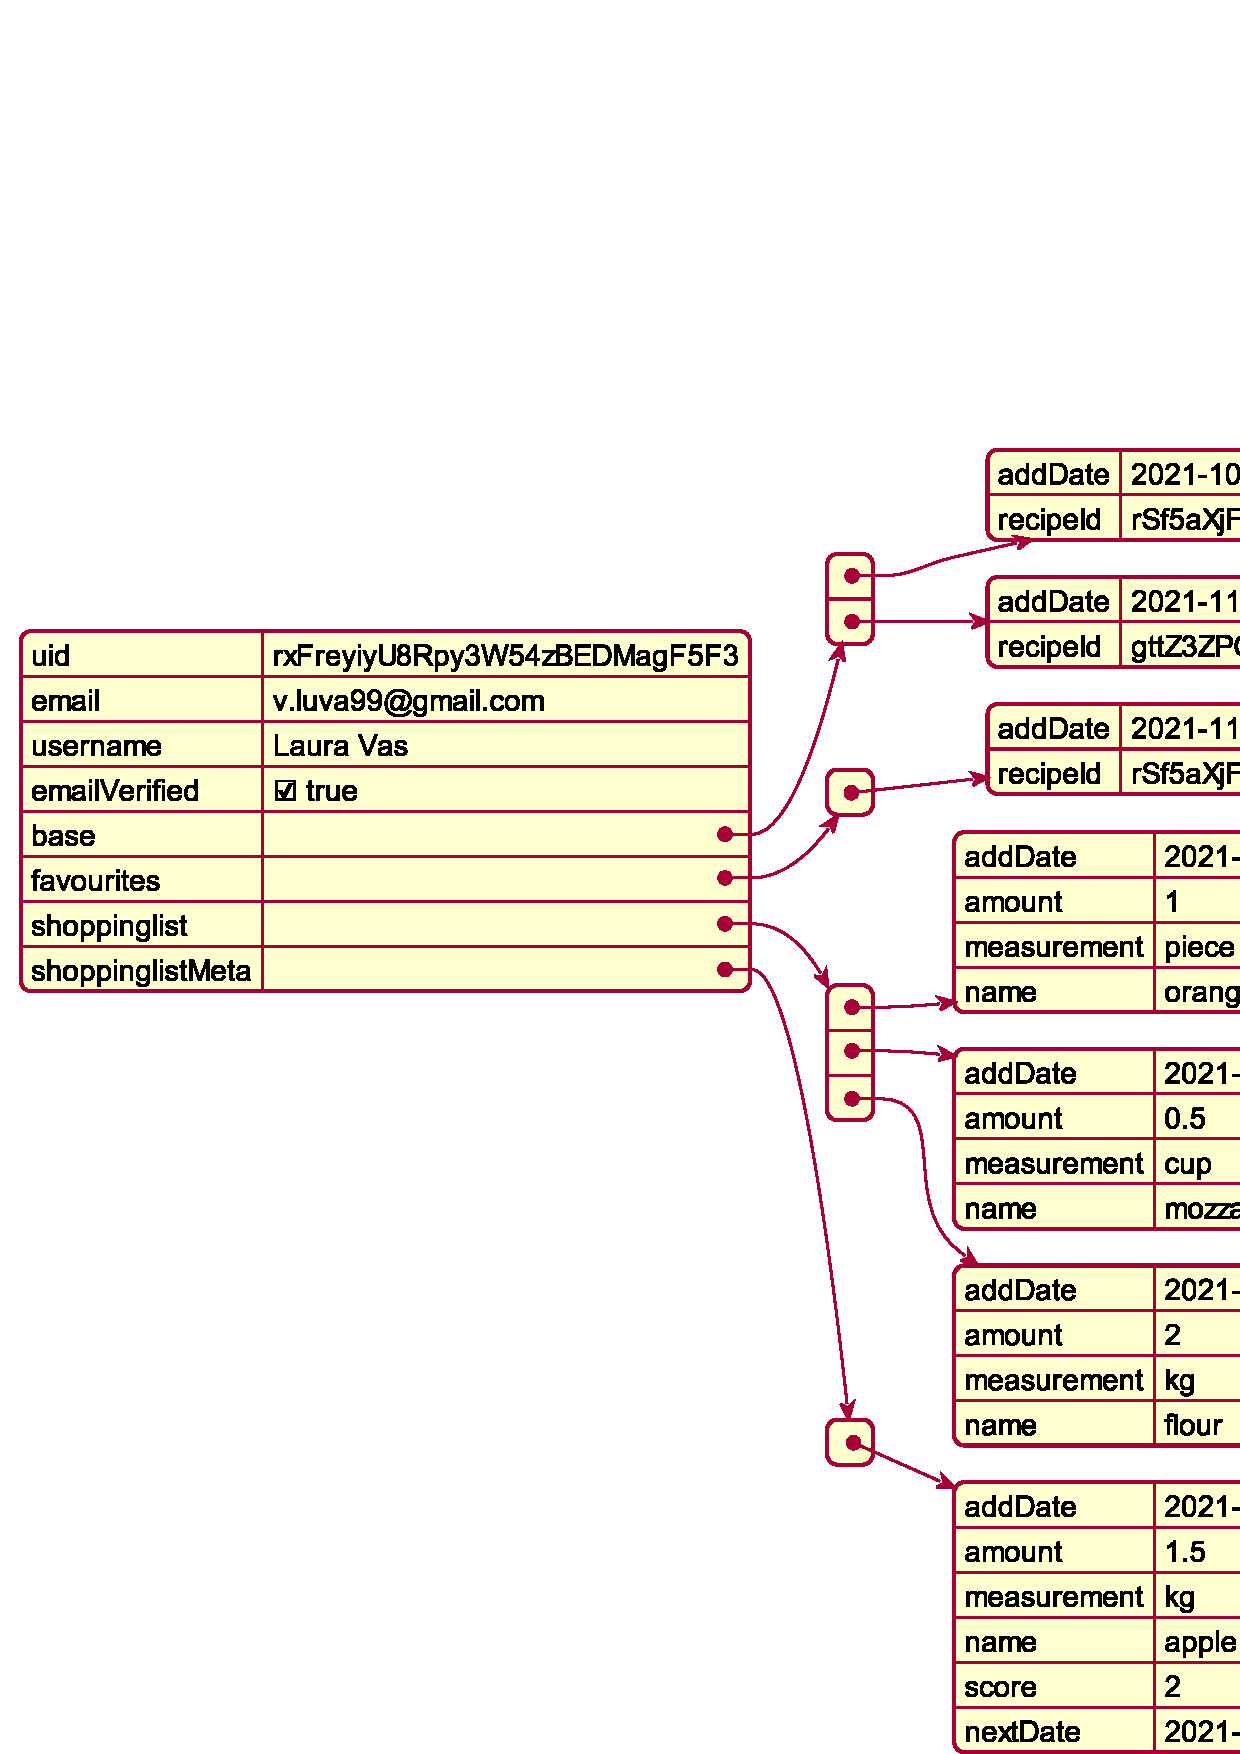
\includegraphics[width=\textwidth]{out/diagrams/jsonUsers/jsonUsers.png}
\begin{figure}[H]
	\centering
	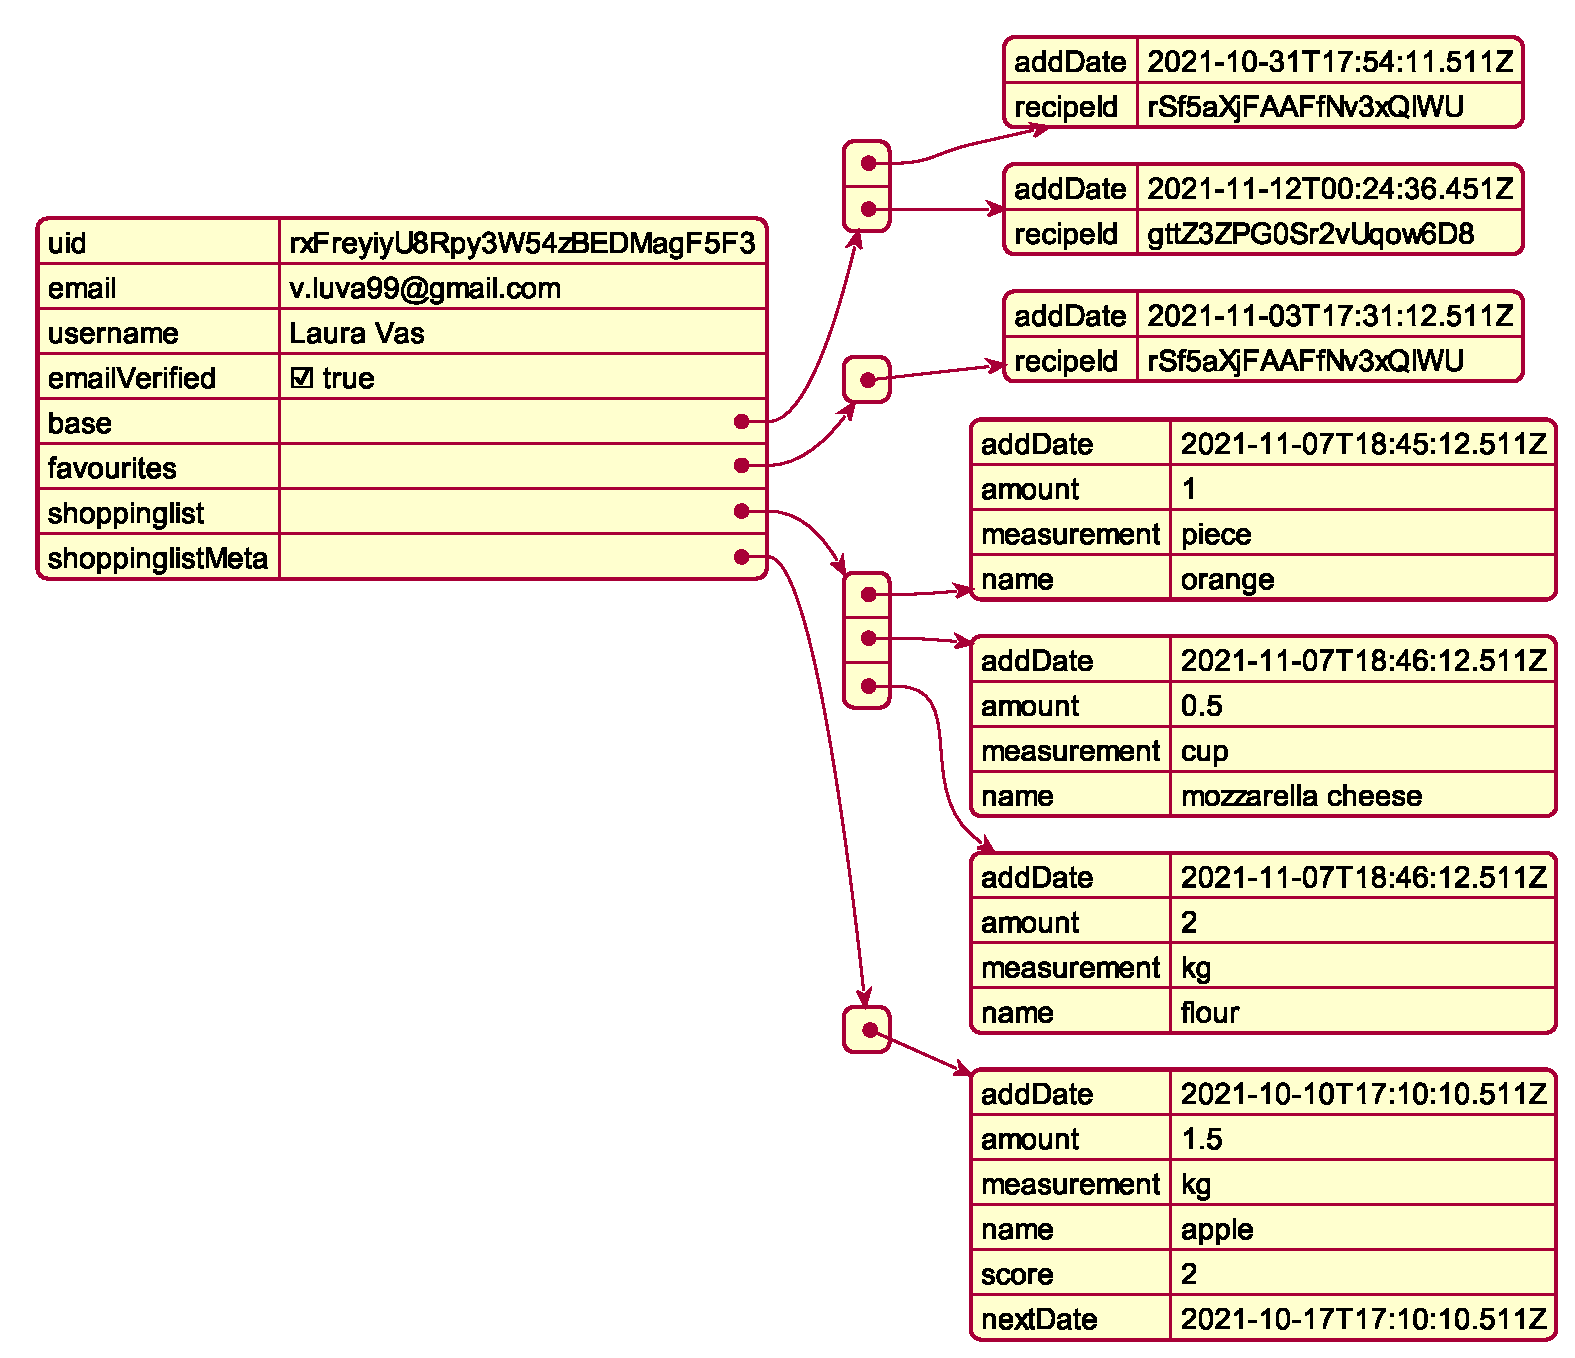
\includegraphics[width=\textwidth]{out/diagrams/jsonUsers/jsonUsers.eps}
	\caption{Egy minta felhaszáló adatairól}
    \label{fig:jsonUsers}
\end{figure}

\section{Reports}
Mivel a weblap úgy lett tervezve, hogy a közösség építi, és mindenki ugyanazokat a recepteket látja, ezért lennie kell egy lehetőségnek, ahol a felhasználók hibát tudnak jelezni és ezeket a hibákat az adatbázisban el kell tudni tárolni. Tehát minden recept végén van lehetőség visszajelzést  küldeni, ha hibás receptet találnak. A bejelenthető hiba típusai fixek, így könnyebben lehet a jövőben megkeresni, hogy mi lehet a hiba az adott recepttel. 

Ezeket a bejelentett hibákat egy kollekcióban tároljuk, ahol minden dokumentum egy-egy bejelentett hibát tárol. A “creationDate” a bejelentés idejét jelzi. A “problem” pedig az opciókból választott a problémát legjobban leíró lehetőség, amit a felhasználó választ. Valamint végül feljegyezzük, hogy melyik receptnél volt ez és hogy ki küldte. A “userId” megegyezik a korábban említett “uid” értékkel a “users” kollekcióból, mivel ez az érték, ami a bejelentkezés során az auth adott a felhasználónak.


\noindent
\begin{figure}[H]
	\centering
	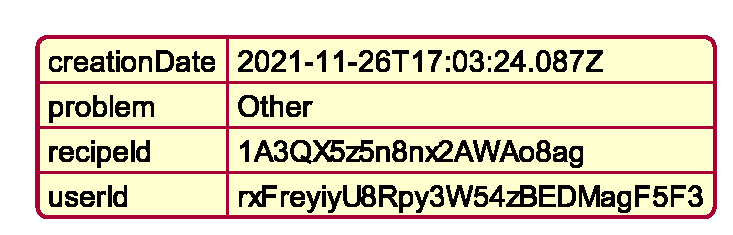
\includegraphics[scale=0.6]{out/diagrams/jsonReports/jsonReports.eps}
	\caption{Egy minta a hiba bejelentésre}
    \label{fig:jsonReports}
\end{figure}

%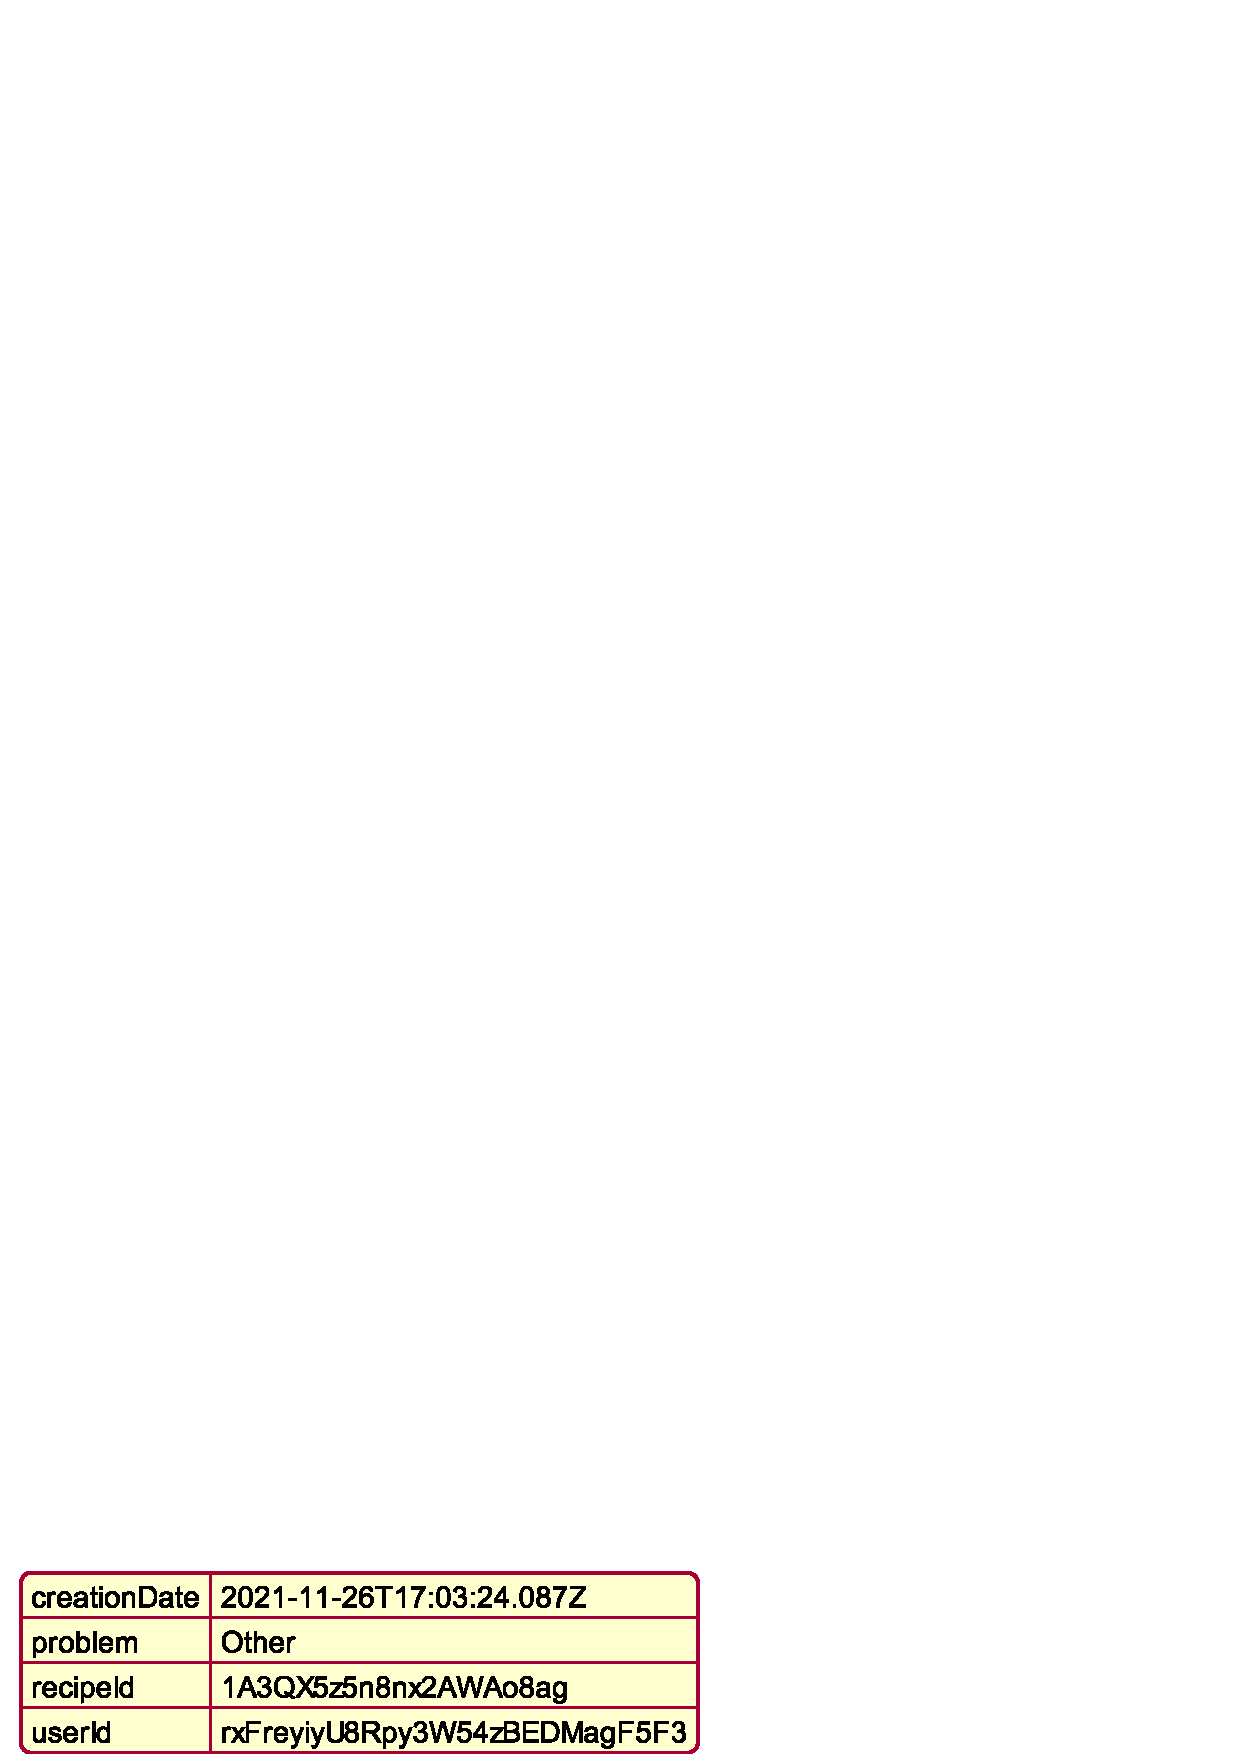
\includegraphics[width=\textwidth]{out/diagrams/jsonReports/jsonReports.png}
%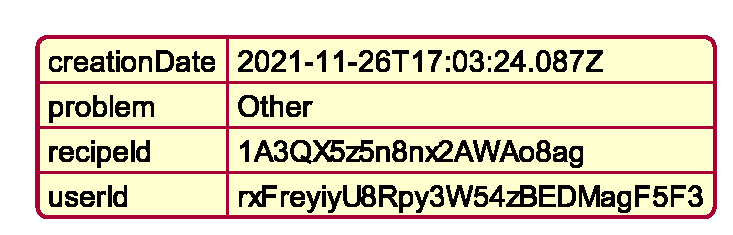
\includegraphics[width=\textwidth]{out/diagrams/jsonReports/jsonReports.eps}


%\chapter{Fontosabb kód részek és ismertetései}
%\section{asd} -> A rendszer magas szintű áttekintése


\chapter{Tesztelés}
A fontosabb funkciók, amik meghatározzák az alap témáját a weblapnak tesztelve lettek. A szerver oldali funkciók mind, az alap működések közé tartoznak,ezért a cloud function moduloknak be lett állítva automatikus tesztelés. Ennek segítségével, ha valami nagyobb változtatást csináltunk,mint például egy rendszer szintű frissítés a FireBase csomagnak, akkor egyszerűen le lehet tesztelni, hogy még minden jól működik-e. Ezt egyszerű unit tesztekkel oldottam meg. A teszteket az npm-ről szedett Jasmine csomaggal készítettem.

\section{Recept importálás URL-en keresztül}
Mivel ez a folyamat modulárisan lett felépítve, ezért minden egyes lépését egyszerű tesztelni. A modulok egyesével és a végeredmény is külön tesztelve van.

\subsection{FetchUrlData}

\subsection{JsonLdExtractor}

\subsection{SeparateIngredients}
Az alapanyag szétválasztás az egyik legkényesebb része a importálás folyamatnak, mivel ebben a részben egy string adatot kell megvizsgálni és különböző adattagokra osztani. Ehhez különböző regex formulák lettek kifejlesztve, hogy a különböző eseteket minél jobban és pontosabban tudjuk feldolgozni. Ehhez, egy egyszerű alap és egy komplexebb teszt készűlt.

Az első célja, hogy le ellenőrizze, hogy a tört szám karakter és egyéb tört szám változatok helyesen vannak átkonvertálva float értékre. A második teszt pedig egy tömböt kap értéknek, amiben rengeteg különböző eset van felsorolva olyan példákkal, amit élő importálás során kaphatunk és szélsőséges probléma lehet. Ezek közé tartozik a három alapeset, ahol vagy szépen visszaadja a mennyiséget, mértékegységet és az alapanyag megnevezését, vagy ha nem talál mértékegységet, de van szám, akkor berendezi, hogy mennyi datab alapanyagot talált, vgay végűl, ha nincs szám se, akkor csak simán visszaadja alapértelmezett módon. Ezen kívül le kell ellenőrizni azokat az eseteket, amik komplexé tették a regex teszteket például, a korábban említett tört karakter helyes észlelése és formázása.

\subsection{ImageDownloader}

\subsection{CalorieCalculator}

\section{GetData}

\chapter{Továbbfejlesztési lehetőségek}
\section{Személyre szabott ajánló}
Mivel a regisztrációnál sok egyéb adat van még eltárolva a felhasználóról, ezért ezeket fel lehet használni, hogy személyre szabott receptajánlója legyen mindenkinek a kezdőoldalon. Ez azt jelenti, hogy felmérést lehet indítani arról, hogy az adatbázisban lévő receptek mely felhasználó csoporthoz vannak leggyakrabban elmentve. Ezeket az adatokat a jövőben fel lehet használni a  receptek kilistázáhához a ajánlóban. 

Amíg a receptet nem mentette ki eléggé sok ember, addig nehéz lehet megállapítani, hogy mely felhasználói csoportoknak tetszhet. Így, ilyenkor a feltöltő csoportjához sorolhatjuk, ezzel is segítve a recept korai javaslását.

\section{Recept ellenőrző admin felület}
Jelenleg már létezik minden recept alatt egy bejelentő mező, ahol hibákat tudnak a felhasználók küldeni a receptek állapotáról. Jelenleg ez még csak el van tárolva az adatbázisban, viszont a jövőben, a könnyű kezelés érdekében ezekhez lehetne csinálni egy adminisztrációs felületet. Ezen az oldalon ki lennének listázva az hibás receptek és az admin egy kattintással rá tud nézni a receptre úgy ahogy a felhasználók is látják.

Itt két lehetősége lenne a hiba megoldására. Ha olyan a recept, hogy nem egyértelmű hogyan lehetne javítani, akkor az törlésre kerül. Ehhez írni kell egy olyan funkciót, ami nemcsak törli az adatbázis receptek kollekciójából, hanem törli,  a felhasználók  recept gyűjteményeiből is. Amennyiben a javítás lehetséges, akkor az admin számára az összes adat módosítható, így könnyen meg tudja tenni a javítást.


\section{Desktop-os és Telefonos kinézet továbbfejlesztése}
Jelenleg a mobilos és desktopos nézetek nem használják ki az adtott platform által nyújtott lehetőségeket tökéletesen. Így például az asztali nézetben sok üres kihasználatlan hely marad, míg bizonyos komponensek a telefonon túl nagyok. Ezeket az alap beviteli komponensek lecserélésével lehetne javítani. Illetve az asztali nézetet esetleg újra gondolni az üres helyeknek új felhasználát kitalálni. 

\section{Mértékegység átváltás}
Mivek két típusú mértékegységeket szokás használni főzésnél, mégpedig az Egyesült Államok által használt rendszert (cup, ounce, inch, stb) vagy az általános SI mértékegységeket (ml, g, dkg, stb.) és konyhai mértékegységeket (tsb, tbsp, stb.). Így a recept nézetben hasznos volna, ha az összetevők mértékegységeit automatikusan át tudná váltani a program. ez azért jutott eszembe mivel, általában az emberek csak az egyiket vagy a másikat ismerik jobban. Tehát be lehetne a profilban beállítani, hogy a felhasználó melyiket preferálja, valamint, hogy akarja-e hogy mindig át legyenek váltva. Ezen kívül lehet még akár minden recept tetején egy gombbal megkérni a weblapot, hogy váltsa át a mértékegységeket.

\section{Főzési folyamat lejátszó}


\section{Videók lejátszása (ha volt a recepthez)}




\chapter*{Nyilatkozat}
%Egy üres sort adunk a tartalomjegyzékhez:
\addtocontents{toc}{\ }
\addcontentsline{toc}{section}{Nyilatkozat}
%\hspace{\parindent}

% A nyilatkozat szövege más titkos és nem titkos dolgozatok esetében.
% Csak az egyik tipusú myilatokzatnak kell a dolgozatban szerepelni
% A ponok helyére az adatok értelemszerűen behelyettesídendők es
% a szakdolgozat /diplomamunka szo megfeleloen kivalasztando.


%A nyilatkozat szövege TITKOSNAK NEM MINŐSÍTETT dolgozatban a következő:
%A pontokkal jelölt szövegrészek értelemszerűen a szövegszerkesztőben és
%nem kézzel helyettesítendők:

\noindent
Alulírott \makebox[4cm]{\dotfill} szakos hallgató, kijelentem, hogy a dolgozatomat a Szegedi Tudományegyetem, Informatikai Intézet \makebox[4cm]{\dotfill} Tanszékén készítettem, \makebox[4cm]{\dotfill} diploma megszerzése érdekében.

Kijelentem, hogy a dolgozatot más szakon korábban nem védtem meg, saját munkám eredménye, és csak a hivatkozott forrásokat (szakirodalom, eszközök, stb.) használtam fel.

Tudomásul veszem, hogy szakdolgozatomat / diplomamunkámat a Szegedi Tudományegyetem Informatikai Intézet könyvtárában, a helyben olvasható könyvek között helyezik el.

\vspace*{2cm}

\begin{tabular}{lc}
	Szeged, \today\
	\hspace{2cm} & \makebox[6cm]{\dotfill} \\
	             & aláírás                 \\
\end{tabular}


\vspace*{4cm}

%A nyilatkozat szövege TITKOSNAK MINŐSÍTETT dolgozatban a következő:

\noindent
Alulírott \makebox[4cm]{\dotfill} szakos hallgató, kijelentem, hogy a dolgozatomat a Szegedi Tudományegyetem, Informatikai Intézet \makebox[4cm]{\dotfill} Tanszékén készítettem, \makebox[4cm]{\dotfill} diploma megszerzése érdekében.

Kijelentem, hogy a dolgozatot más szakon korábban nem védtem meg, saját munkám eredménye, és csak a hivatkozott forrásokat (szakirodalom, eszközök, stb.) használtam fel.

Tudomásul veszem, hogy szakdolgozatomat / diplomamunkámat a TVSZ 4. sz. mellékletében leírtak szerint kezelik.

\vspace*{2cm}

\begin{tabular}{lc}
	Szeged, \today\
	\hspace{2cm} & \makebox[6cm]{\dotfill} \\
	             & aláírás                 \\
\end{tabular}





\chapter*{Köszönetnyilvánítás}
\addcontentsline{toc}{section}{Köszönetnyilvánítás}

Ezúton szeretnék köszönetet mondani \textbf{X. Y-nak} ezért és ezért \ldots


%% Az itrodalomjegyzek keszitheto a BibTeX segedprogrammal:
%\bibliography{diploma}
%\bibliographystyle{plain}

%VAGY "kézzel" a következő módon:

\begin{thebibliography}{9}
	%10-nél kevesebb hivatkozás esetén

	%\begin{thebibliography}{99}
	% 10-nél több hivatkozás esetén

	\addcontentsline{toc}{section}{Irodalomjegyzék}

	%Elso szerzok vezetekneve alapjan ábécérendben rendezve.


	%folyóirat cikk: szerzok(k), a folyóirat neve kiemelve,
	%az evfolyam felkoveren, zarojelben az evszam, vegul az oldalszamok es pont.
	\bibitem{Gischer}
	J. L. Gischer,
	The equational theory of pomsets.
	\emph{Theoret. Comput. Sci.}, \textbf{61}(1988), 199--224.

	%könyv (szerzo(k), a könyv neve kiemelve, utana a kiado, a kiado szekhelye, az evszam es pont.)
	\bibitem{Pin}
	J.-E. Pin,
	\emph{Varieties of Formal Languages},
	Plenum Publishing Corp., New York, 1986.





\end{thebibliography}




\end{document}
